\documentclass[11pt]{article}

    \usepackage[breakable]{tcolorbox}
    \usepackage{parskip} % Stop auto-indenting (to mimic markdown behaviour)
    
    \usepackage{iftex}
    \ifPDFTeX
    	\usepackage[T1]{fontenc}
    	\usepackage{mathpazo}
    \else
    	\usepackage{fontspec}
    \fi

    % Basic figure setup, for now with no caption control since it's done
    % automatically by Pandoc (which extracts ![](path) syntax from Markdown).
    \usepackage{graphicx}
    % Maintain compatibility with old templates. Remove in nbconvert 6.0
    \let\Oldincludegraphics\includegraphics
    % Ensure that by default, figures have no caption (until we provide a
    % proper Figure object with a Caption API and a way to capture that
    % in the conversion process - todo).
    \usepackage{caption}
    \DeclareCaptionFormat{nocaption}{}
    \captionsetup{format=nocaption,aboveskip=0pt,belowskip=0pt}
    \usepackage[portuguese]{babel}
    \usepackage[Export]{adjustbox} % Used to constrain images to a maximum size
    \adjustboxset{max size={0.9\linewidth}{0.9\paperheight}}
    \usepackage{float}
    \floatplacement{figure}{H} % forces figures to be placed at the correct location
    \usepackage{xcolor} % Allow colors to be defined
    \usepackage{enumerate} % Needed for markdown enumerations to work
    \usepackage{geometry} % Used to adjust the document margins
    \usepackage{amsmath} % Equations
    \usepackage{amssymb} % Equations
    \usepackage{textcomp} % defines textquotesingle
    % Hack from http://tex.stackexchange.com/a/47451/13684:
    \AtBeginDocument{%
        \def\PYZsq{\textquotesingle}% Upright quotes in Pygmentized code
    }
    \usepackage{upquote} % Upright quotes for verbatim code
    \usepackage{eurosym} % defines \euro
    \usepackage[mathletters]{ucs} % Extended unicode (utf-8) support
    \usepackage{fancyvrb} % verbatim replacement that allows latex
    \usepackage{grffile} % extends the file name processing of package graphics 
                         % to support a larger range
    \makeatletter % fix for grffile with XeLaTeX
    \def\Gread@@xetex#1{%
      \IfFileExists{"\Gin@base".bb}%
      {\Gread@eps{\Gin@base.bb}}%
      {\Gread@@xetex@aux#1}%
    }
    \makeatother

    % The hyperref package gives us a pdf with properly built
    % internal navigation ('pdf bookmarks' for the table of contents,
    % internal cross-reference links, web links for URLs, etc.)
    \usepackage{hyperref}
    % The default LaTeX title has an obnoxious amount of whitespace. By default,
    % titling removes some of it. It also provides customization options.
    \usepackage{titling}
    \usepackage{longtable} % longtable support required by pandoc >1.10
    \usepackage{booktabs}  % table support for pandoc > 1.12.2
    \usepackage[inline]{enumitem} % IRkernel/repr support (it uses the enumerate* environment)
    \usepackage[normalem]{ulem} % ulem is needed to support strikethroughs (\sout)
                                % normalem makes italics be italics, not underlines
    \usepackage{mathrsfs}
    

    
    % Colors for the hyperref package
    \definecolor{urlcolor}{rgb}{0,.145,.698}
    \definecolor{linkcolor}{rgb}{.29,.32,.58}
    \definecolor{citecolor}{rgb}{.12,.54,.11}

    % ANSI colors
    \definecolor{ansi-black}{HTML}{3E424D}
    \definecolor{ansi-black-intense}{HTML}{282C36}
    \definecolor{ansi-red}{HTML}{E75C58}
    \definecolor{ansi-red-intense}{HTML}{B22B31}
    \definecolor{ansi-green}{HTML}{00A250}
    \definecolor{ansi-green-intense}{HTML}{007427}
    \definecolor{ansi-yellow}{HTML}{DDB62B}
    \definecolor{ansi-yellow-intense}{HTML}{B27D12}
    \definecolor{ansi-blue}{HTML}{208FFB}
    \definecolor{ansi-blue-intense}{HTML}{0065CA}
    \definecolor{ansi-magenta}{HTML}{D160C4}
    \definecolor{ansi-magenta-intense}{HTML}{A03196}
    \definecolor{ansi-cyan}{HTML}{60C6C8}
    \definecolor{ansi-cyan-intense}{HTML}{258F8F}
    \definecolor{ansi-white}{HTML}{C5C1B4}
    \definecolor{ansi-white-intense}{HTML}{A1A6B2}
    \definecolor{ansi-default-inverse-fg}{HTML}{FFFFFF}
    \definecolor{ansi-default-inverse-bg}{HTML}{000000}

    % commands and environments needed by pandoc snippets
    % extracted from the output of `pandoc -s`
    \providecommand{\tightlist}{%
      \setlength{\itemsep}{0pt}\setlength{\parskip}{0pt}}
    \DefineVerbatimEnvironment{Highlighting}{Verbatim}{commandchars=\\\{\}}
    % Add ',fontsize=\small' for more characters per line
    \newenvironment{Shaded}{}{}
    \newcommand{\KeywordTok}[1]{\textcolor[rgb]{0.00,0.44,0.13}{\textbf{{#1}}}}
    \newcommand{\DataTypeTok}[1]{\textcolor[rgb]{0.56,0.13,0.00}{{#1}}}
    \newcommand{\DecValTok}[1]{\textcolor[rgb]{0.25,0.63,0.44}{{#1}}}
    \newcommand{\BaseNTok}[1]{\textcolor[rgb]{0.25,0.63,0.44}{{#1}}}
    \newcommand{\FloatTok}[1]{\textcolor[rgb]{0.25,0.63,0.44}{{#1}}}
    \newcommand{\CharTok}[1]{\textcolor[rgb]{0.25,0.44,0.63}{{#1}}}
    \newcommand{\StringTok}[1]{\textcolor[rgb]{0.25,0.44,0.63}{{#1}}}
    \newcommand{\CommentTok}[1]{\textcolor[rgb]{0.38,0.63,0.69}{\textit{{#1}}}}
    \newcommand{\OtherTok}[1]{\textcolor[rgb]{0.00,0.44,0.13}{{#1}}}
    \newcommand{\AlertTok}[1]{\textcolor[rgb]{1.00,0.00,0.00}{\textbf{{#1}}}}
    \newcommand{\FunctionTok}[1]{\textcolor[rgb]{0.02,0.16,0.49}{{#1}}}
    \newcommand{\RegionMarkerTok}[1]{{#1}}
    \newcommand{\ErrorTok}[1]{\textcolor[rgb]{1.00,0.00,0.00}{\textbf{{#1}}}}
    \newcommand{\NormalTok}[1]{{#1}}
    
    % Additional commands for more recent versions of Pandoc
    \newcommand{\ConstantTok}[1]{\textcolor[rgb]{0.53,0.00,0.00}{{#1}}}
    \newcommand{\SpecialCharTok}[1]{\textcolor[rgb]{0.25,0.44,0.63}{{#1}}}
    \newcommand{\VerbatimStringTok}[1]{\textcolor[rgb]{0.25,0.44,0.63}{{#1}}}
    \newcommand{\SpecialStringTok}[1]{\textcolor[rgb]{0.73,0.40,0.53}{{#1}}}
    \newcommand{\ImportTok}[1]{{#1}}
    \newcommand{\DocumentationTok}[1]{\textcolor[rgb]{0.73,0.13,0.13}{\textit{{#1}}}}
    \newcommand{\AnnotationTok}[1]{\textcolor[rgb]{0.38,0.63,0.69}{\textbf{\textit{{#1}}}}}
    \newcommand{\CommentVarTok}[1]{\textcolor[rgb]{0.38,0.63,0.69}{\textbf{\textit{{#1}}}}}
    \newcommand{\VariableTok}[1]{\textcolor[rgb]{0.10,0.09,0.49}{{#1}}}
    \newcommand{\ControlFlowTok}[1]{\textcolor[rgb]{0.00,0.44,0.13}{\textbf{{#1}}}}
    \newcommand{\OperatorTok}[1]{\textcolor[rgb]{0.40,0.40,0.40}{{#1}}}
    \newcommand{\BuiltInTok}[1]{{#1}}
    \newcommand{\ExtensionTok}[1]{{#1}}
    \newcommand{\PreprocessorTok}[1]{\textcolor[rgb]{0.74,0.48,0.00}{{#1}}}
    \newcommand{\AttributeTok}[1]{\textcolor[rgb]{0.49,0.56,0.16}{{#1}}}
    \newcommand{\InformationTok}[1]{\textcolor[rgb]{0.38,0.63,0.69}{\textbf{\textit{{#1}}}}}
    \newcommand{\WarningTok}[1]{\textcolor[rgb]{0.38,0.63,0.69}{\textbf{\textit{{#1}}}}}
    
    
    % Define a nice break command that doesn't care if a line doesn't already
    % exist.
    \def\br{\hspace*{\fill} \\* }
    % Math Jax compatibility definitions
    \def\gt{>}
    \def\lt{<}
    \let\Oldtex\TeX
    \let\Oldlatex\LaTeX
    \renewcommand{\TeX}{\textrm{\Oldtex}}
    \renewcommand{\LaTeX}{\textrm{\Oldlatex}}
    % Document parameters
    % Document title
    \title{Final}
    
    
    
    
    
% Pygments definitions
\makeatletter
\def\PY@reset{\let\PY@it=\relax \let\PY@bf=\relax%
    \let\PY@ul=\relax \let\PY@tc=\relax%
    \let\PY@bc=\relax \let\PY@ff=\relax}
\def\PY@tok#1{\csname PY@tok@#1\endcsname}
\def\PY@toks#1+{\ifx\relax#1\empty\else%
    \PY@tok{#1}\expandafter\PY@toks\fi}
\def\PY@do#1{\PY@bc{\PY@tc{\PY@ul{%
    \PY@it{\PY@bf{\PY@ff{#1}}}}}}}
\def\PY#1#2{\PY@reset\PY@toks#1+\relax+\PY@do{#2}}

\@namedef{PY@tok@w}{\def\PY@tc##1{\textcolor[rgb]{0.73,0.73,0.73}{##1}}}
\@namedef{PY@tok@c}{\let\PY@it=\textit\def\PY@tc##1{\textcolor[rgb]{0.25,0.50,0.50}{##1}}}
\@namedef{PY@tok@cp}{\def\PY@tc##1{\textcolor[rgb]{0.74,0.48,0.00}{##1}}}
\@namedef{PY@tok@k}{\let\PY@bf=\textbf\def\PY@tc##1{\textcolor[rgb]{0.00,0.50,0.00}{##1}}}
\@namedef{PY@tok@kp}{\def\PY@tc##1{\textcolor[rgb]{0.00,0.50,0.00}{##1}}}
\@namedef{PY@tok@kt}{\def\PY@tc##1{\textcolor[rgb]{0.69,0.00,0.25}{##1}}}
\@namedef{PY@tok@o}{\def\PY@tc##1{\textcolor[rgb]{0.40,0.40,0.40}{##1}}}
\@namedef{PY@tok@ow}{\let\PY@bf=\textbf\def\PY@tc##1{\textcolor[rgb]{0.67,0.13,1.00}{##1}}}
\@namedef{PY@tok@nb}{\def\PY@tc##1{\textcolor[rgb]{0.00,0.50,0.00}{##1}}}
\@namedef{PY@tok@nf}{\def\PY@tc##1{\textcolor[rgb]{0.00,0.00,1.00}{##1}}}
\@namedef{PY@tok@nc}{\let\PY@bf=\textbf\def\PY@tc##1{\textcolor[rgb]{0.00,0.00,1.00}{##1}}}
\@namedef{PY@tok@nn}{\let\PY@bf=\textbf\def\PY@tc##1{\textcolor[rgb]{0.00,0.00,1.00}{##1}}}
\@namedef{PY@tok@ne}{\let\PY@bf=\textbf\def\PY@tc##1{\textcolor[rgb]{0.82,0.25,0.23}{##1}}}
\@namedef{PY@tok@nv}{\def\PY@tc##1{\textcolor[rgb]{0.10,0.09,0.49}{##1}}}
\@namedef{PY@tok@no}{\def\PY@tc##1{\textcolor[rgb]{0.53,0.00,0.00}{##1}}}
\@namedef{PY@tok@nl}{\def\PY@tc##1{\textcolor[rgb]{0.63,0.63,0.00}{##1}}}
\@namedef{PY@tok@ni}{\let\PY@bf=\textbf\def\PY@tc##1{\textcolor[rgb]{0.60,0.60,0.60}{##1}}}
\@namedef{PY@tok@na}{\def\PY@tc##1{\textcolor[rgb]{0.49,0.56,0.16}{##1}}}
\@namedef{PY@tok@nt}{\let\PY@bf=\textbf\def\PY@tc##1{\textcolor[rgb]{0.00,0.50,0.00}{##1}}}
\@namedef{PY@tok@nd}{\def\PY@tc##1{\textcolor[rgb]{0.67,0.13,1.00}{##1}}}
\@namedef{PY@tok@s}{\def\PY@tc##1{\textcolor[rgb]{0.73,0.13,0.13}{##1}}}
\@namedef{PY@tok@sd}{\let\PY@it=\textit\def\PY@tc##1{\textcolor[rgb]{0.73,0.13,0.13}{##1}}}
\@namedef{PY@tok@si}{\let\PY@bf=\textbf\def\PY@tc##1{\textcolor[rgb]{0.73,0.40,0.53}{##1}}}
\@namedef{PY@tok@se}{\let\PY@bf=\textbf\def\PY@tc##1{\textcolor[rgb]{0.73,0.40,0.13}{##1}}}
\@namedef{PY@tok@sr}{\def\PY@tc##1{\textcolor[rgb]{0.73,0.40,0.53}{##1}}}
\@namedef{PY@tok@ss}{\def\PY@tc##1{\textcolor[rgb]{0.10,0.09,0.49}{##1}}}
\@namedef{PY@tok@sx}{\def\PY@tc##1{\textcolor[rgb]{0.00,0.50,0.00}{##1}}}
\@namedef{PY@tok@m}{\def\PY@tc##1{\textcolor[rgb]{0.40,0.40,0.40}{##1}}}
\@namedef{PY@tok@gh}{\let\PY@bf=\textbf\def\PY@tc##1{\textcolor[rgb]{0.00,0.00,0.50}{##1}}}
\@namedef{PY@tok@gu}{\let\PY@bf=\textbf\def\PY@tc##1{\textcolor[rgb]{0.50,0.00,0.50}{##1}}}
\@namedef{PY@tok@gd}{\def\PY@tc##1{\textcolor[rgb]{0.63,0.00,0.00}{##1}}}
\@namedef{PY@tok@gi}{\def\PY@tc##1{\textcolor[rgb]{0.00,0.63,0.00}{##1}}}
\@namedef{PY@tok@gr}{\def\PY@tc##1{\textcolor[rgb]{1.00,0.00,0.00}{##1}}}
\@namedef{PY@tok@ge}{\let\PY@it=\textit}
\@namedef{PY@tok@gs}{\let\PY@bf=\textbf}
\@namedef{PY@tok@gp}{\let\PY@bf=\textbf\def\PY@tc##1{\textcolor[rgb]{0.00,0.00,0.50}{##1}}}
\@namedef{PY@tok@go}{\def\PY@tc##1{\textcolor[rgb]{0.53,0.53,0.53}{##1}}}
\@namedef{PY@tok@gt}{\def\PY@tc##1{\textcolor[rgb]{0.00,0.27,0.87}{##1}}}
\@namedef{PY@tok@err}{\def\PY@bc##1{{\setlength{\fboxsep}{\string -\fboxrule}\fcolorbox[rgb]{1.00,0.00,0.00}{1,1,1}{\strut ##1}}}}
\@namedef{PY@tok@kc}{\let\PY@bf=\textbf\def\PY@tc##1{\textcolor[rgb]{0.00,0.50,0.00}{##1}}}
\@namedef{PY@tok@kd}{\let\PY@bf=\textbf\def\PY@tc##1{\textcolor[rgb]{0.00,0.50,0.00}{##1}}}
\@namedef{PY@tok@kn}{\let\PY@bf=\textbf\def\PY@tc##1{\textcolor[rgb]{0.00,0.50,0.00}{##1}}}
\@namedef{PY@tok@kr}{\let\PY@bf=\textbf\def\PY@tc##1{\textcolor[rgb]{0.00,0.50,0.00}{##1}}}
\@namedef{PY@tok@bp}{\def\PY@tc##1{\textcolor[rgb]{0.00,0.50,0.00}{##1}}}
\@namedef{PY@tok@fm}{\def\PY@tc##1{\textcolor[rgb]{0.00,0.00,1.00}{##1}}}
\@namedef{PY@tok@vc}{\def\PY@tc##1{\textcolor[rgb]{0.10,0.09,0.49}{##1}}}
\@namedef{PY@tok@vg}{\def\PY@tc##1{\textcolor[rgb]{0.10,0.09,0.49}{##1}}}
\@namedef{PY@tok@vi}{\def\PY@tc##1{\textcolor[rgb]{0.10,0.09,0.49}{##1}}}
\@namedef{PY@tok@vm}{\def\PY@tc##1{\textcolor[rgb]{0.10,0.09,0.49}{##1}}}
\@namedef{PY@tok@sa}{\def\PY@tc##1{\textcolor[rgb]{0.73,0.13,0.13}{##1}}}
\@namedef{PY@tok@sb}{\def\PY@tc##1{\textcolor[rgb]{0.73,0.13,0.13}{##1}}}
\@namedef{PY@tok@sc}{\def\PY@tc##1{\textcolor[rgb]{0.73,0.13,0.13}{##1}}}
\@namedef{PY@tok@dl}{\def\PY@tc##1{\textcolor[rgb]{0.73,0.13,0.13}{##1}}}
\@namedef{PY@tok@s2}{\def\PY@tc##1{\textcolor[rgb]{0.73,0.13,0.13}{##1}}}
\@namedef{PY@tok@sh}{\def\PY@tc##1{\textcolor[rgb]{0.73,0.13,0.13}{##1}}}
\@namedef{PY@tok@s1}{\def\PY@tc##1{\textcolor[rgb]{0.73,0.13,0.13}{##1}}}
\@namedef{PY@tok@mb}{\def\PY@tc##1{\textcolor[rgb]{0.40,0.40,0.40}{##1}}}
\@namedef{PY@tok@mf}{\def\PY@tc##1{\textcolor[rgb]{0.40,0.40,0.40}{##1}}}
\@namedef{PY@tok@mh}{\def\PY@tc##1{\textcolor[rgb]{0.40,0.40,0.40}{##1}}}
\@namedef{PY@tok@mi}{\def\PY@tc##1{\textcolor[rgb]{0.40,0.40,0.40}{##1}}}
\@namedef{PY@tok@il}{\def\PY@tc##1{\textcolor[rgb]{0.40,0.40,0.40}{##1}}}
\@namedef{PY@tok@mo}{\def\PY@tc##1{\textcolor[rgb]{0.40,0.40,0.40}{##1}}}
\@namedef{PY@tok@ch}{\let\PY@it=\textit\def\PY@tc##1{\textcolor[rgb]{0.25,0.50,0.50}{##1}}}
\@namedef{PY@tok@cm}{\let\PY@it=\textit\def\PY@tc##1{\textcolor[rgb]{0.25,0.50,0.50}{##1}}}
\@namedef{PY@tok@cpf}{\let\PY@it=\textit\def\PY@tc##1{\textcolor[rgb]{0.25,0.50,0.50}{##1}}}
\@namedef{PY@tok@c1}{\let\PY@it=\textit\def\PY@tc##1{\textcolor[rgb]{0.25,0.50,0.50}{##1}}}
\@namedef{PY@tok@cs}{\let\PY@it=\textit\def\PY@tc##1{\textcolor[rgb]{0.25,0.50,0.50}{##1}}}

\def\PYZbs{\char`\\}
\def\PYZus{\char`\_}
\def\PYZob{\char`\{}
\def\PYZcb{\char`\}}
\def\PYZca{\char`\^}
\def\PYZam{\char`\&}
\def\PYZlt{\char`\<}
\def\PYZgt{\char`\>}
\def\PYZsh{\char`\#}
\def\PYZpc{\char`\%}
\def\PYZdl{\char`\$}
\def\PYZhy{\char`\-}
\def\PYZsq{\char`\'}
\def\PYZdq{\char`\"}
\def\PYZti{\char`\~}
% for compatibility with earlier versions
\def\PYZat{@}
\def\PYZlb{[}
\def\PYZrb{]}
\makeatother


    % For linebreaks inside Verbatim environment from package fancyvrb. 
    \makeatletter
        \newbox\Wrappedcontinuationbox 
        \newbox\Wrappedvisiblespacebox 
        \newcommand*\Wrappedvisiblespace {\textcolor{red}{\textvisiblespace}} 
        \newcommand*\Wrappedcontinuationsymbol {\textcolor{red}{\llap{\tiny$\m@th\hookrightarrow$}}} 
        \newcommand*\Wrappedcontinuationindent {3ex } 
        \newcommand*\Wrappedafterbreak {\kern\Wrappedcontinuationindent\copy\Wrappedcontinuationbox} 
        % Take advantage of the already applied Pygments mark-up to insert 
        % potential linebreaks for TeX processing. 
        %        {, <, #, %, $, ' and ": go to next line. 
        %        _, }, ^, &, >, - and ~: stay at end of broken line. 
        % Use of \textquotesingle for straight quote. 
        \newcommand*\Wrappedbreaksatspecials {% 
            \def\PYGZus{\discretionary{\char`\_}{\Wrappedafterbreak}{\char`\_}}% 
            \def\PYGZob{\discretionary{}{\Wrappedafterbreak\char`\{}{\char`\{}}% 
            \def\PYGZcb{\discretionary{\char`\}}{\Wrappedafterbreak}{\char`\}}}% 
            \def\PYGZca{\discretionary{\char`\^}{\Wrappedafterbreak}{\char`\^}}% 
            \def\PYGZam{\discretionary{\char`\&}{\Wrappedafterbreak}{\char`\&}}% 
            \def\PYGZlt{\discretionary{}{\Wrappedafterbreak\char`\<}{\char`\<}}% 
            \def\PYGZgt{\discretionary{\char`\>}{\Wrappedafterbreak}{\char`\>}}% 
            \def\PYGZsh{\discretionary{}{\Wrappedafterbreak\char`\#}{\char`\#}}% 
            \def\PYGZpc{\discretionary{}{\Wrappedafterbreak\char`\%}{\char`\%}}% 
            \def\PYGZdl{\discretionary{}{\Wrappedafterbreak\char`\$}{\char`\$}}% 
            \def\PYGZhy{\discretionary{\char`\-}{\Wrappedafterbreak}{\char`\-}}% 
            \def\PYGZsq{\discretionary{}{\Wrappedafterbreak\textquotesingle}{\textquotesingle}}% 
            \def\PYGZdq{\discretionary{}{\Wrappedafterbreak\char`\"}{\char`\"}}% 
            \def\PYGZti{\discretionary{\char`\~}{\Wrappedafterbreak}{\char`\~}}% 
        } 
        % Some characters . , ; ? ! / are not pygmentized. 
        % This macro makes them "active" and they will insert potential linebreaks 
        \newcommand*\Wrappedbreaksatpunct {% 
            \lccode`\~`\.\lowercase{\def~}{\discretionary{\hbox{\char`\.}}{\Wrappedafterbreak}{\hbox{\char`\.}}}% 
            \lccode`\~`\,\lowercase{\def~}{\discretionary{\hbox{\char`\,}}{\Wrappedafterbreak}{\hbox{\char`\,}}}% 
            \lccode`\~`\;\lowercase{\def~}{\discretionary{\hbox{\char`\;}}{\Wrappedafterbreak}{\hbox{\char`\;}}}% 
            \lccode`\~`\:\lowercase{\def~}{\discretionary{\hbox{\char`\:}}{\Wrappedafterbreak}{\hbox{\char`\:}}}% 
            \lccode`\~`\?\lowercase{\def~}{\discretionary{\hbox{\char`\?}}{\Wrappedafterbreak}{\hbox{\char`\?}}}% 
            \lccode`\~`\!\lowercase{\def~}{\discretionary{\hbox{\char`\!}}{\Wrappedafterbreak}{\hbox{\char`\!}}}% 
            \lccode`\~`\/\lowercase{\def~}{\discretionary{\hbox{\char`\/}}{\Wrappedafterbreak}{\hbox{\char`\/}}}% 
            \catcode`\.\active
            \catcode`\,\active 
            \catcode`\;\active
            \catcode`\:\active
            \catcode`\?\active
            \catcode`\!\active
            \catcode`\/\active 
            \lccode`\~`\~ 	
        }
    \makeatother

    \let\OriginalVerbatim=\Verbatim
    \makeatletter
    \renewcommand{\Verbatim}[1][1]{%
        %\parskip\z@skip
        \sbox\Wrappedcontinuationbox {\Wrappedcontinuationsymbol}%
        \sbox\Wrappedvisiblespacebox {\FV@SetupFont\Wrappedvisiblespace}%
        \def\FancyVerbFormatLine ##1{\hsize\linewidth
            \vtop{\raggedright\hyphenpenalty\z@\exhyphenpenalty\z@
                \doublehyphendemerits\z@\finalhyphendemerits\z@
                \strut ##1\strut}%
        }%
        % If the linebreak is at a space, the latter will be displayed as visible
        % space at end of first line, and a continuation symbol starts next line.
        % Stretch/shrink are however usually zero for typewriter font.
        \def\FV@Space {%
            \nobreak\hskip\z@ plus\fontdimen3\font minus\fontdimen4\font
            \discretionary{\copy\Wrappedvisiblespacebox}{\Wrappedafterbreak}
            {\kern\fontdimen2\font}%
        }%
        
        % Allow breaks at special characters using \PYG... macros.
        \Wrappedbreaksatspecials
        % Breaks at punctuation characters . , ; ? ! and / need catcode=\active 	
        \OriginalVerbatim[#1,codes*=\Wrappedbreaksatpunct]%
    }
    \makeatother

    % Exact colors from NB
    \definecolor{incolor}{HTML}{303F9F}
    \definecolor{outcolor}{HTML}{D84315}
    \definecolor{cellborder}{HTML}{CFCFCF}
    \definecolor{cellbackground}{HTML}{F7F7F7}
    
    % prompt
    \makeatletter
    \newcommand{\boxspacing}{\kern\kvtcb@left@rule\kern\kvtcb@boxsep}
    \makeatother
    \newcommand{\prompt}[4]{
        \ttfamily\llap{{\color{#2}[#3]:\hspace{3pt}#4}}\vspace{-\baselineskip}
    }
    

    
    % Prevent overflowing lines due to hard-to-break entities
    \sloppy 
    % Setup hyperref package
    \hypersetup{
      breaklinks=true,  % so long urls are correctly broken across lines
      colorlinks=true,
      urlcolor=urlcolor,
      linkcolor=linkcolor,
      citecolor=citecolor,
      }
    % Slightly bigger margins than the latex defaults
    
    \geometry{verbose,tmargin=1in,bmargin=1in,lmargin=1in,rmargin=1in}
    
    \title{Aplicação do Algoritmo \emph{Google PageRank}
em Páginas do
Wikipédia}
    \author{Eduardo Adame Salles \and Rodrigo Gomes Hutz Pintucci}
    \date{17 de Novembro de 2021}

\begin{document}
    
    
    \begin{titlepage}
	\centering
	
\includegraphics[width=0.45\textwidth]{emap_logo.png}\par\vspace{1cm}
	\vspace{1.5cm}
	{\huge\bfseries Aplicação do Algoritmo \emph{Google PageRank}
        em Páginas do
        Wikipédia\par}
	\vspace{2cm}
	{\Large\itshape Eduardo Adame Salles \\ Rodrigo Gomes Hutz Pintucci \par}
	\vfill
	sob orientação de\par
	Yuri Fahham \textsc{Saporito}

	\vfill

    % Bottom of the page
	{\large 17 de Novembro de 2021 \par}
    \end{titlepage}
    
    \tableofcontents
    
    \pagenumbering{Roman}
    \setcounter{page}{1}
   
    \newpage
    \pagenumbering{arabic}
    \setcounter{page}{1}
\hypertarget{introduuxe7uxe3o}{%
\section{Introdução}\label{introduuxe7uxe3o}}

Este relatório tem como objetivo apresentar diversas abordagens do
PageRank tais como: o contexto no qual fora criado, o desenvolvimento de
seu algorítmo, sua implementação em \emph{Python} e sua aplicação em um
conjunto de dados criado a partir de \emph{web scraping}. O
\emph{Google PageRank} foi uma solução desenvolvida principalmente por
Larry Page, co-fundador do \emph{Google}, para solucionar problemas
relacionados a indexação de websites. Desde então, esse algoritmo ganhou
muita notoriedade e mérito por ser eficaz e veloz. Sua implementação, de
modo geral, utiliza conceitos discutidos durante a disciplina de Álgebra
Linear, para qual esse relatório é dedicado.

Para a utilização de \emph{web scraping}, nós utilizaremos ferramentas
modernas em \emph{Python} para adquirir e armazenar dados da Wikipédia,
criando nossa ``micro internet''. O trabalho todo é baseado em
notebooks, utilizando como módulo principal o \texttt{numpy} e suas
funções do \texttt{numpy.linalg}, além do \texttt{pandas} e \texttt{bs4}
para a aquisição do conjunto de dados.


    \hypertarget{a-motivauxe7uxe3o}{%
\section{A Motivação}\label{a-motivauxe7uxe3o}}

Desde que a Internet tornou-se amplamente acessível, motores de busca
foram criados, com o intuito de facilitar a procura de informação.
Contudo, apenas uma lista com todos os demais sites não é o suficiente:
idealmente, os resultados devem ser dispostos de forma eficiente, na
qual opções cuja relevância atendem melhor o usuário são apresentados
com maior destaque. Decorrente disso, muitas empresas foram criadas com
o objetivo de estruturar um algoritmo rápido e eficaz.

    \hypertarget{google}{%
\subsection{\texorpdfstring{\emph{Google}}{Google}}\label{google}}

Dentre essas empresas, foi criada o \emph{Google}, em janeiro de 1996. O
\emph{Google} foi projetado por dois estudantes da Universidade de
Stanford, localizada na Califórnia: Larry Page e Sergey Brin; com uma
missão: organizar a informação mundial e torná-la acessível e útil. No
mercado da época, já existiam alguns buscadores, tais como
\emph{Wandex}, \emph{WebCrawler} e \emph{Dogpile}. O que Larry e Sergey
perceberam, entretanto, foi que esses buscadores convencionais
utilizavam como parâmetro a contagem de vezes que os termos de buscas
eram presentes na primeira página, e que esse era possível o
desenvolvimento de um melhor método. Assim, iniciaram uma tecnologia que
fosse capaz de analisar a relação entre os sites, cujo nome é uma
homenagem a seu criador e uma referência ao termo \textit{web page}: o \emph{PageRank}.

    \hypertarget{pagerank}{%
\subsection{PageRank}\label{pagerank}}

Através da Internet, temos acesso a uma grande teia de documentos
inter-relacionados de hipertextos, denominada \emph{World Wide Web}
(WWW). O diferencial presente no algoritmo de \emph{PageRank} e a grande
sacada de seus criadores é que essa interconectividade poderia e deveria
ser um fator importantíssimo para o ranqueamento de sites. Dessa forma,
ao invés da quantidade de termos de busca, a relevância de um site é
baseada com relação a quantidade e importância de outros, aqueles
capazes de realizar uma ligação de volta ao site original.

    \hypertarget{outras-aplicauxe7uxf5es}{%
\subsection{Outras aplicações}\label{outras-aplicauxe7uxf5es}}

Por mais que seja comumente associado à sua finalidade original de
ranquear páginas para o \emph{Google}, o algoritmo matemático pode ser
utilizado em qualquer tipo de rede ou grafo. Alguns usos atuais para o
\emph{PageRank} se encontram em:

\begin{itemize}
\item Bibliometria
\item Previsões e recomendações de links
\item Análise de sistemas de redes rodoviárias
\item Predição do número de pessoas em certas ruas e espaços.
\item Análise de redes sociais e de informações
\begin{itemize}
\item O \emph{Twitter} utiliza do algoritmo para apresentar aos usuários outras contas relevantes.
\end{itemize}
\item Ciências tais como biologia, química, física e neurocîencia.
\begin{itemize}
\item Na biologia, é utilizado na análise de redes de proteína.
\item Na ecologia, uma versão do algoritmo pode determinar quais espécies são essencias para um ecossistema.
\item Na neurociência, temos em uma rede neural a correlação do
\emph{PageRank} de um neurônio com sua taxa de disparo relativa.
\end{itemize}
\item Outras áreas
\begin{itemize}
\item Nos esportes, já foi utilizado para ranquear a
performance de times e jogadores, tais como os times da \emph{National
Football League}, dos Estados Unidos.
\item Na semântica lexical, foi
utilizado para performar desambiguação e similaridade de semântica.
\end{itemize}
\end{itemize}

\newpage

    \hypertarget{o-algoritmo}{%
\section{O Algoritmo}\label{o-algoritmo}}

Para compreender como o \emph{PageRank} funciona, vamos examinar uma
situação onde nossa rede é composta de apenas 4 sites: \(A\), \(B\),
\(C\) e \(D\) e temos um hipotético usuário que caminha de um site para
o outro sem preferências. Uma característica dessa tecnologia é que a
soma de todos os \emph{PageRank} é \(1\). Portanto, inicialmente, todos
tem \emph{PageRank} igual a \(0,25\).

\begin{figure}
\centering
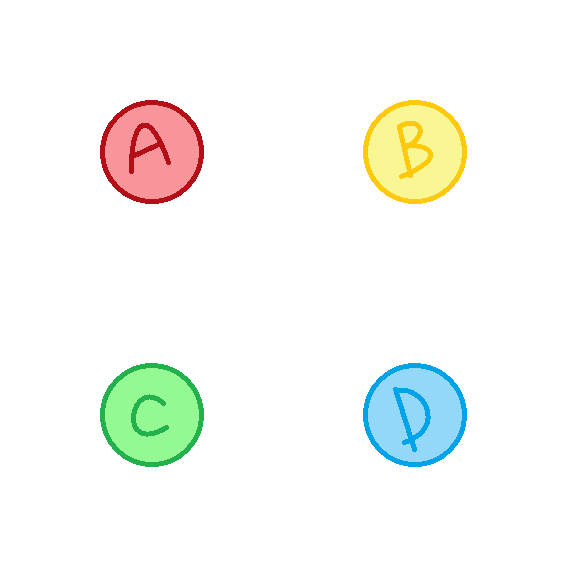
\includegraphics[width = .4\textwidth]{../img/ABCD1.png}
\end{figure}


    Vamos supor agora que eles estejam conectados de alguma forma entre si.
Para melhor visualização, as conexões de um site consigo mesmo e o
caminho de duas vias foi oculto. Nessa primeira situação, os sites
\(B\), \(C\) e \(D\) resultam unicamente em \(A\). Assim, o
\emph{PageRank} de \(A\) pode ser calculado como a soma do
\emph{PageRank} dos demais sites:

\begin{figure}
\centering
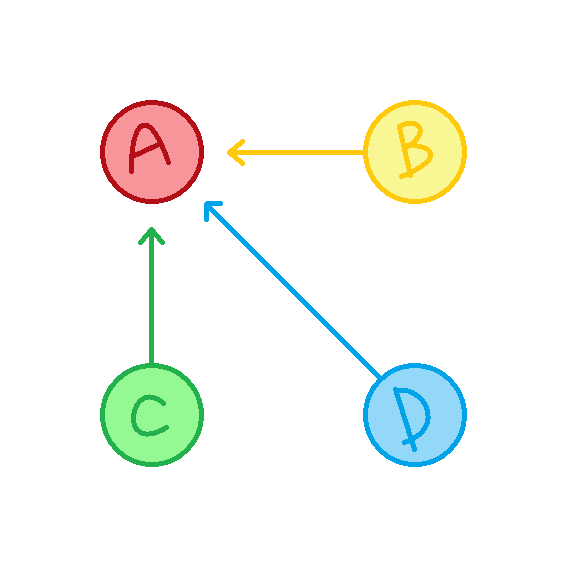
\includegraphics[width = .4\textwidth]{../img/ABCD2.png}
\end{figure}

\[PR(A) = PR(B) + PR(C) + PR(D)\]

\newpage

    Contudo, geralmente os sites não apontam para um único local. Portanto,
vamos supor que os sites \(B\), \(C\) e \(D\) também tem conexões entre
si.

\begin{figure}
\centering
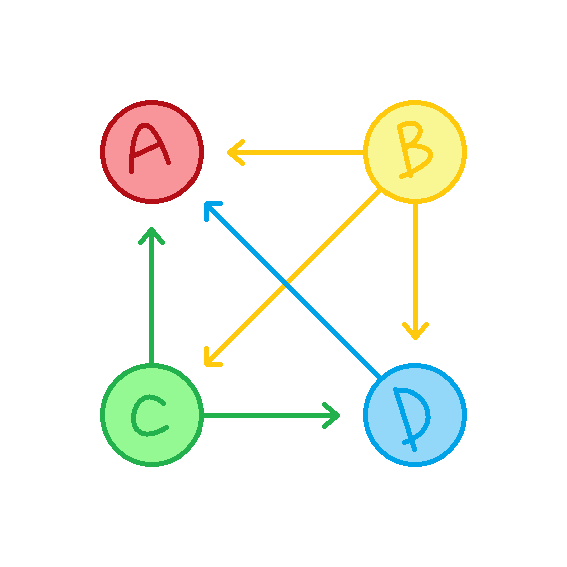
\includegraphics[width = .4\textwidth]{../img/ABCD3.png}
\end{figure}

Observe que o site \(B\) tem 3 conexões, enquanto o site \(C\) tem 2
conexões e o site \(D\) apenas 1. Voltemos a nosso hipotético usuário:
caso ele se encontre no site \(C\), pode tanto ir para \(A\) quanto para
\(D\). Como ele não possui preferências, a chance para que vá para um
desses sites é igual. Dessa forma, no cálculo do \emph{PageRank} de
\(A\), já não podemos considerar o valor total do \emph{PageRank} de
\(C\); e sim apenas metade. O mesmo ocorre para o valor proveniente do
\emph{PageRank} de \(B\). Nessa situação, o valor proveniente de \(D\)
permanece o mesmo pois possui apenas uma conexão. Portanto, temos:

\[PR(A) = \displaystyle \frac{PR(B)}{3} + \frac{PR(C)}{2} + \frac{PR(D)}{1}\]

    Podemos, então, generalizar essa conta: o \emph{PageRank} de um site vai
ser a soma entre a razão do \emph{PageRank} de sites que referenciam o
site original e o número de ligações contidos nesses outros sites.
Assim, considerando o número de ligações do site \(B\) o número \(L(B)\)
temos:
\[PR(A) = \displaystyle \frac{PR(B)}{L(B)} + \frac{PR(C)}{L(C)} + \frac{PR(D)}{L(D)}\]
Para um número qualquer de sites, podemos utilizar a seguinte notação de
somatória:
\[{\displaystyle PR(u)=\sum _{v\in B_{u}}{\frac {PR(v)}{L(v)}}}\] (sendo
\(B_u\) o conjunto de páginas que referenciam \(u\))

\newpage

    \hypertarget{erros}{%
\subsection{Erros}\label{erros}}

O sistema descrito é funcional para a maioria das situações. Porém, duas
situações devem ser consideradas: a drenagem e o ciclo.

    Voltemos na segunda imagem. Como descrito anteriormente, as ligações
saindo de \(A\) e as ligações de um site consigo mesmo foram ocultadas.
Vamos supor, entretanto, que as ligações saindo de \(A\) não foram
ocultadas, e sim que realmente não existem. Dessa forma, o usuário
hipotético entraria eventualmente em \(A\) e seria incapaz de sair. Se
analisarmos o \emph{PageRank}, notaríamos que \(A\) causou uma drenagem
nos demais valores.

\begin{figure}
\centering
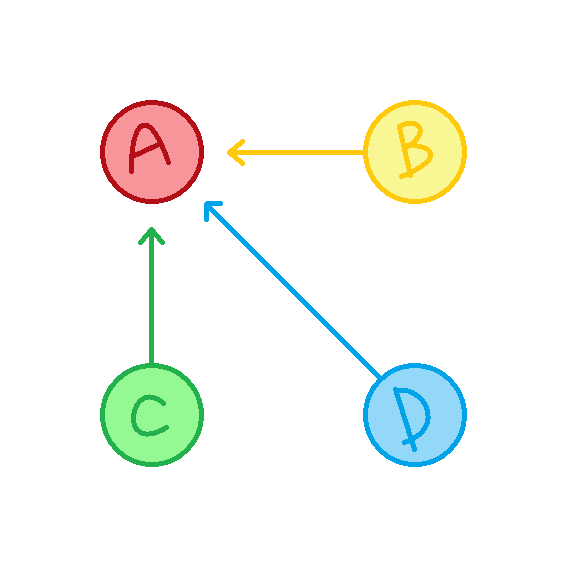
\includegraphics[width = .4\textwidth]{../img/ABCD2.png}
\end{figure}

    A outra situação é quando temos um ciclo fechado, onde cada site possui
uma unica ligação e eventualmente chegamos no site inicial.

\begin{figure}
\centering
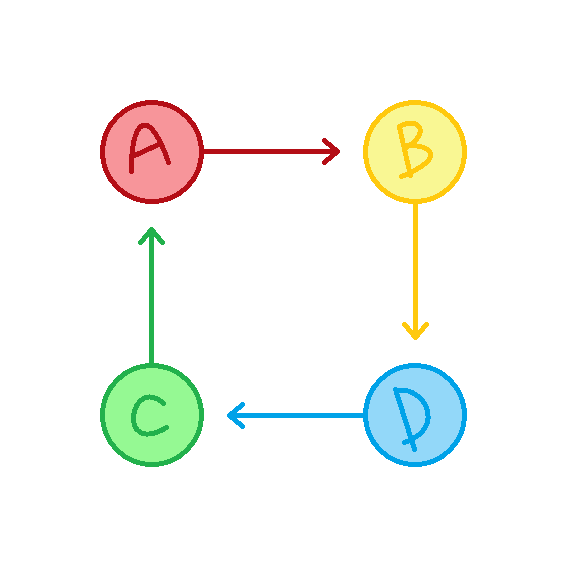
\includegraphics[width = .4\textwidth]{../img/ABCD4.png}
\end{figure}

Nesse caso, temos que \(A\) aponta somente para \(B\), que por sua vez aponta
somente para \(C\), que aponta somente para \(D\) e que por fim aponta
somente para \(A\). Assim, o nosso usuário hipotético fica preso nesse
ciclo infinito.

    \hypertarget{a-soluuxe7uxe3o}{%
\subsection{A solução}\label{a-soluuxe7uxe3o}}

Para solucionar esses erros, adicionamos uma ideia em nosso algoritmo: a
que o usuário hipotético pode cansar de ir para para outro site a partir
de uma referência e, a qualquer momento, pode visitar qualquer site, sem
preferência. Portanto, denominamos de \(d\) um fator de amortecimento: a
probabilidade, contida entre 0 e 1, de que o usuário irá seguir a ideia
inicial apresentada.

    Analogamente, temos que a probabilidade de que o usuário decida acessar
qualquer site aleatoriamente será de \((1 - d)\). Como definimos que é
aleatório, a chance para cada site nessa segunda escolha é equivalente,
e portanto temos \(\frac{(1 - d)}{N}\), sendo \(N\) o número total de
sites.\\
Concluímos assim que o cálculo do \emph{PageRank} pode ser dado da
seguinte maneira:
\[PR(p_i) = \displaystyle \frac{(1 - d)}{N} + d{\sum _{p_j\in M{p_i}}{\frac {PR(p_j)}{L(p_j)}}}\]
(com \(M(p_i)\) sendo o conjunto de páginas que referenciam \(p_i\))

    \hypertarget{pagerank-como-um-problema-de-uxe1lgebra-linear}{%
\subsection{\texorpdfstring{\emph{PageRank} como um problema de
Álgebra
Linear}{PageRank como um problema de Álgebra Linear}}\label{pagerank-como-um-problema-de-uxe1lgebra-linear}}

Vamos agora analisar como podemos utilizar de matrizes para facilitar o
cálculo de nosso algoritmo. O primeiro passo será transformar o cálculo
genérico numa linguagem vetorial, para que tenhamos simultaneamente o
cálculo de todos os \emph{PageRanks}. Assim, denominamos \(\mathbf {R}\)
o vetor contendo o \emph{PageRank} dos sites \(p_1\) até \(p_n\).

    Voltando ao nosso exemplo composto de 4 sites mais simples, no qual
ainda não havia o fator de amortecimento, temos que
\(PR(A) = \frac{PR(B)}{L(B)} + \frac{PR(C)}{L(C)} + \frac{PR(D)}{L(D)}\).
Podemos reescrever esse segundo membro como o resultado de um produto
entre o vetor linha
\(\begin{bmatrix}\frac{1}{L(B)} & \frac{1}{L(C)} & \frac{1}{L(D)}\end{bmatrix}\)
e o vetor coluna \(\mathbf {R}\), o que novamente equivale a \(PR(A)\).
Agora, imagine que pegamos todos os vetores linhas para os demais sites
e montamos uma matriz \(\mathcal {M}\). O resultado do produto dessa
matriz agora não seria mais \(PR(A)\), e sim um vetor composto de todos
os \emph{PageRanks}: o vetor \(\mathbf {R}\).

    Porém, dois pontos devem ser levados em consideração: o primeiro, é que
um site pode não ter referência para outro, e o segundo é que o fator de
amortecimento está ausente da equação. Para o primeiro ponto, vamos
alterar a matriz \(\mathcal {M}\) para que cada elemento seja uma função
do tipo \(\ell(p_i,p_j)\), que pode assumir dois valores: 0, caso não
haja referência de \(p_j\) para \(p_i\), ou \(\frac{1}{L(p_j)}\) caso
haja. Para o segundo ponto, basta multiplicar a matriz \(\mathcal {M}\)
pelo fator de amortecimento \(d\) e adicionar um vetor coluna de tamanho
n composto de elementos \(\frac{(1-d)}{N}\) Assim, temos o seguinte
resultado:

\[{\displaystyle \mathbf {R} = \begin{bmatrix}PR(p_{1})\\PR(p_{2})\\\vdots \\PR(p_{N})\end{bmatrix}  ={\begin{bmatrix}{(1-d)/N}\\{(1-d)/N}\\\vdots \\{(1-d)/N}\end{bmatrix}}+d{\begin{bmatrix}\ell (p_{1},p_{1})&\ell (p_{1},p_{2})&\cdots &\ell (p_{1},p_{N})\\\ell (p_{2},p_{1})&\ddots &&\vdots \\\vdots &&\ell (p_{i},p_{j})&\\\ell (p_{N},p_{1})&\cdots &&\ell (p_{N},p_{N})\end{bmatrix}}\mathbf {R} }\]

    Se tirarmos em evidência \(\frac{(1-d)}{N}\) do primeiro vetor, temos um
vetor composto apenas de 1. Podemos aproveitar o fato de que todos os
\emph{PageRanks} somam 1 para reescrever esse vetor como o produto
\(\mathbf {ER}\), sendo \(\mathbf {E}\) um matriz composta apenas de 1,
ou seja:

\[\displaystyle \begin{bmatrix}{(1-d)/N}\\{(1-d)/N}\\\vdots \\{(1-d)/N}\end{bmatrix} = \frac{(1-d)}{N}\begin{bmatrix}{1}\\{1}\\\vdots \\{1}\end{bmatrix} = \frac{(1-d)}{N}ER\]

    Dessa forma, todos os termos estão multiplicados pelo vetor coluna
\(R\), de forma que podemos mais uma vez tirar o fator em evidência:

\[\displaystyle \mathbf {R} = (\frac{(1-d)}{N}\mathbf {E} + d \mathcal {M}) \mathbf {R}\]

    Se chamarmos \((\frac{(1-d)}{N}\mathbf {E} + d \mathcal {M})\) de
\(\widehat {\mathcal {M}}\), temos:
\[\displaystyle \mathbf {R} = \widehat {\mathcal {M}} \mathbf {R}\] De
onde tiramos que \(\mathbf{R}\) \textbf{é um autovetor de}
\(\widehat {\mathcal {M}}\) \textbf{para o autovalor 1}.

    Temos que os elementos da matriz \(\widehat {\mathcal {M}}\) são
não-negativos e que suas colunas somam 1 (ou em alguns casos raros, 0).
Dessa forma, essa matriz é estotástica, ou seja, seu maior autovalor é
1. Conseguimos concluir assim que a matriz \(\mathbf{R}\) de
\emph{PageRank} é o \textbf{autovetor do maior autovalor} da matriz
\(\widehat {\mathcal {M}}\).

    Portanto, um método para o cálculo de \emph{PageRank} é: 1. Descobrir os
autovalores da matriz \(\widehat {\mathcal {M}}\). 2. Encontrar, dentre
eles, o maior. 3. Encontrar o autovetor para esse autovalor.

Contudo, esse método não é usual para matrizes muito grandes, pois
demanda bastante poder computacional para descobrir todos seus
autovalores.

    \hypertarget{muxe9todo-das-potuxeancias}{%
\subsection{Método das potências}\label{muxe9todo-das-potuxeancias}}

Podemos, contudo, utilizar das equações que encontramos para calcular um
método de aproximar o vetor de \emph{PageRank} sem ter de calcular os
autovalores da matriz. Quando se tem uma matriz \(A\) tal que um de seus
autovalores é estritamente maior que os outros e temos um vetor \(b_0\)
que tem um componente não-nulo na direção do autovetor relacionado ao
maior autovalores, temos a seguinte propriedade, denominada \emph{Power
Method} ou \emph{Power Iteration}:
\[{\displaystyle b_{k+1}={\frac {Ab_{k}}{\|Ab_{k}\|}}}\] Onde o vetor
\(b_0\) converge para o autovetor relacionado ao maior autovalor de
\(A\). Isso ocorre quando ele é multiplicado pela matriz, normalizado e
o processo é repetido uma certa quantidade de vezes.

    Devido às propriedades da matriz \(\widehat {\mathcal {M}}\)
(estocástica, primitiva e irredutível), e sabendo que \(R\) é justamente
o autovetor relacionado ao maior autovalor dessa matriz, sabemos que
podemos então utilizar esse método para aproximar o valor de
\(\mathbf{R}\) sem ter de calcular todos os autovalores. Essas
propriedades também fazem com que não seja necessário normalizar cada
iteração, uma vez que esta etapa serve apenas para evitar um crescimento
descontrolado do vetor.

    Podemos iniciar com um vetor \(\mathbf{R}_0\), onde as entradas são
equivalentes; de valor \(\frac{1}{N}\), sendo \(N\) o número total de
sites. Assim, escrevemos:
\[{\displaystyle \mathbf{R}_{k+1}={\widehat {\mathcal {M}}}\mathbf{R}_k}\]

    Fazendo isso, podemos comparar a norma da diferença entre
\(\mathbf{R}_{k+1}\) e \(\mathbf{R}_k\) até que ele seja menor que um
valor escolhido muito pequeno. Se tivermos
\(\displaystyle |\mathbf{R}_{k+1}-\mathbf{R}_k| \lt\epsilon\), então
sabemos que os valores de \(\mathbf{R}_{k+1}\) convergiram para valores
muitos próximos ao do vetor \(\mathbf{R}\) encontrado pelo método do
autovetor.

    Logo, encontramos os dois métodos que estaremos utilizando e comparando.

    \hypertarget{implementauxe7uxe3o-computacional}{%
\section{Implementação
computacional}\label{implementauxe7uxe3o-computacional}}

Agora, vamos ver como podemos automatizar a execução do algortimo
através de programação. Nesse caso, iremos utilizar o \emph{Python}.
Entretanto, é necessário primeiro importar sua biblioteca \texttt{numpy}
para podermos trabalhar com matrizes.

    \begin{tcolorbox}[breakable, size=fbox, boxrule=1pt, pad at break*=1mm,colback=cellbackground, colframe=cellborder]
\prompt{In}{incolor}{1}{\boxspacing}
\begin{Verbatim}[commandchars=\\\{\}]
\PY{k+kn}{import} \PY{n+nn}{numpy} \PY{k}{as} \PY{n+nn}{np}
\PY{k+kn}{import} \PY{n+nn}{numpy}\PY{n+nn}{.}\PY{n+nn}{linalg} \PY{k}{as} \PY{n+nn}{la}
\end{Verbatim}
\end{tcolorbox}

    Isto feito, podemos criar as funções que serão utilizadas. Inicialmente,
mostraremos o funcionamento em uma matriz gerada automaticamente.
Eventualmente, estaremos utilizando redes retiradas da Internet. \#\#\#
Gerando uma matriz

    \begin{tcolorbox}[breakable, size=fbox, boxrule=1pt, pad at break*=1mm,colback=cellbackground, colframe=cellborder]
\prompt{In}{incolor}{2}{\boxspacing}
\begin{Verbatim}[commandchars=\\\{\}]
\PY{k}{def} \PY{n+nf}{fake\PYZus{}internet}\PY{p}{(}\PY{n}{n}\PY{p}{)}\PY{p}{:}
    \PY{c+c1}{\PYZsh{}\PYZsh{}\PYZsh{}\PYZsh{}\PYZsh{}\PYZsh{}\PYZsh{}\PYZsh{}\PYZsh{}\PYZsh{}\PYZsh{}\PYZsh{}\PYZsh{}\PYZsh{}\PYZsh{}\PYZsh{}\PYZsh{}\PYZsh{}\PYZsh{}\PYZsh{}\PYZsh{}\PYZsh{}\PYZsh{}\PYZsh{}\PYZsh{}\PYZsh{}\PYZsh{}\PYZsh{}\PYZsh{}}
    \PY{c+c1}{\PYZsh{}\PYZsh{}\PYZsh{} CRIA MATRIZ APLICÁVEL \PYZsh{}\PYZsh{}\PYZsh{}}
    \PY{c+c1}{\PYZsh{}\PYZsh{}\PYZsh{}\PYZsh{}\PYZsh{}\PYZsh{}\PYZsh{}\PYZsh{}\PYZsh{}\PYZsh{}\PYZsh{}\PYZsh{}\PYZsh{}\PYZsh{}\PYZsh{}\PYZsh{}\PYZsh{}\PYZsh{}\PYZsh{}\PYZsh{}\PYZsh{}\PYZsh{}\PYZsh{}\PYZsh{}\PYZsh{}\PYZsh{}\PYZsh{}\PYZsh{}\PYZsh{}}
    
    \PY{c+c1}{\PYZsh{} Cria matriz do tamanho n x n com colunas de 0, 1, ..., n\PYZhy{}1.}
    \PY{n}{c} \PY{o}{=} \PY{n}{np}\PY{o}{.}\PY{n}{full}\PY{p}{(}\PY{p}{[}\PY{n}{n}\PY{p}{,}\PY{n}{n}\PY{p}{]}\PY{p}{,} \PY{n}{np}\PY{o}{.}\PY{n}{arange}\PY{p}{(}\PY{n}{n}\PY{p}{)}\PY{p}{)}
    
    \PY{c+c1}{\PYZsh{} Transforma a matriz em booleanos aleatórios com base na desigualdade abaixo.}
    \PY{n}{c} \PY{o}{=} \PY{p}{(}\PY{n+nb}{abs}\PY{p}{(}\PY{n}{np}\PY{o}{.}\PY{n}{random}\PY{o}{.}\PY{n}{standard\PYZus{}cauchy}\PY{p}{(}\PY{p}{[}\PY{n}{n}\PY{p}{,}\PY{n}{n}\PY{p}{]}\PY{p}{)}\PY{o}{/}\PY{l+m+mi}{2}\PY{p}{)} \PY{o}{\PYZgt{}} \PY{p}{(}\PY{n}{np}\PY{o}{.}\PY{n}{abs}\PY{p}{(}\PY{n}{c} \PY{o}{\PYZhy{}} \PY{n}{c}\PY{o}{.}\PY{n}{T}\PY{p}{)} \PY{o}{+} \PY{l+m+mi}{1}\PY{p}{)}\PY{p}{)}
    
    \PY{c+c1}{\PYZsh{} Transforma True em conexões e depois faz as colunas somarem 1.}
    \PY{n}{c} \PY{o}{=} \PY{p}{(}\PY{n}{c}\PY{o}{+}\PY{l+m+mf}{1e\PYZhy{}10}\PY{p}{)} \PY{o}{/} \PY{n}{np}\PY{o}{.}\PY{n}{sum}\PY{p}{(}\PY{p}{(}\PY{n}{c}\PY{o}{+}\PY{l+m+mf}{1e\PYZhy{}10}\PY{p}{)}\PY{p}{,} \PY{n}{axis}\PY{o}{=}\PY{l+m+mi}{0}\PY{p}{)}
    \PY{k}{return} \PY{n}{c}
\end{Verbatim}
\end{tcolorbox}

    Assim, criamos uma matriz quadrada do tamanho que quisermos na qual as
colunas somam 1. Portanto, é uma candidata funcional para a aplicação
dos métodos de \emph{PageRank} que visualizamos. Vamos criar uma
variável \texttt{matrix} para guardar o valor da Internet que criamos.

    \begin{tcolorbox}[breakable, size=fbox, boxrule=1pt, pad at break*=1mm,colback=cellbackground, colframe=cellborder]
\prompt{In}{incolor}{3}{\boxspacing}
\begin{Verbatim}[commandchars=\\\{\}]
\PY{n}{matrix} \PY{o}{=} \PY{n}{fake\PYZus{}internet}\PY{p}{(}\PY{l+m+mi}{4}\PY{p}{)}
\PY{n}{matrix}
\end{Verbatim}
\end{tcolorbox}

            \begin{tcolorbox}[breakable, size=fbox, boxrule=.5pt, pad at break*=1mm, opacityfill=0]
\prompt{Out}{outcolor}{3}{\boxspacing}
\begin{Verbatim}[commandchars=\\\{\}]
array([[2.5e-01, 1.0e-10, 5.0e-01, 5.0e-11],
       [2.5e-01, 1.0e-10, 5.0e-11, 5.0e-11],
       [2.5e-01, 1.0e+00, 5.0e-11, 5.0e-01],
       [2.5e-01, 1.0e-10, 5.0e-01, 5.0e-01]])
\end{Verbatim}
\end{tcolorbox}
        
    Agora, o primeiro método que foi explicado: vamos calcular todos os
autovalores e autovetores presentes na matriz criada. Depois,
organizamos os autovalores em ordem decrescente e utilizamos esta mesma
ordem para os autovetores. Podemos, portanto, remover o primeiro
autovetor dessa lista: será o autovetor correspondente ao maior
autovelor, e portanto, o \emph{PageRank} da matriz. \#\#\# Utilizando os
algoritmos

    \begin{tcolorbox}[breakable, size=fbox, boxrule=1pt, pad at break*=1mm,colback=cellbackground, colframe=cellborder]
\prompt{In}{incolor}{4}{\boxspacing}
\begin{Verbatim}[commandchars=\\\{\}]
\PY{k}{def} \PY{n+nf}{eigPageRank}\PY{p}{(}\PY{n}{linkMatrix}\PY{p}{)}\PY{p}{:}
    \PY{c+c1}{\PYZsh{}\PYZsh{}\PYZsh{}\PYZsh{}\PYZsh{}\PYZsh{}\PYZsh{}\PYZsh{}\PYZsh{}\PYZsh{}\PYZsh{}\PYZsh{}\PYZsh{}\PYZsh{}\PYZsh{}\PYZsh{}\PYZsh{}\PYZsh{}\PYZsh{}\PYZsh{}\PYZsh{}\PYZsh{}\PYZsh{}\PYZsh{}\PYZsh{}\PYZsh{}\PYZsh{}\PYZsh{}\PYZsh{}\PYZsh{}\PYZsh{}\PYZsh{}}
    \PY{c+c1}{\PYZsh{}\PYZsh{}\PYZsh{} PAGERANK POR AUTOVETORES \PYZsh{}\PYZsh{}\PYZsh{}}
    \PY{c+c1}{\PYZsh{}\PYZsh{}\PYZsh{}\PYZsh{}\PYZsh{}\PYZsh{}\PYZsh{}\PYZsh{}\PYZsh{}\PYZsh{}\PYZsh{}\PYZsh{}\PYZsh{}\PYZsh{}\PYZsh{}\PYZsh{}\PYZsh{}\PYZsh{}\PYZsh{}\PYZsh{}\PYZsh{}\PYZsh{}\PYZsh{}\PYZsh{}\PYZsh{}\PYZsh{}\PYZsh{}\PYZsh{}\PYZsh{}\PYZsh{}\PYZsh{}\PYZsh{}}
    
    \PY{c+c1}{\PYZsh{} Calcula os autovalores e autovetores}
    \PY{n}{eVals}\PY{p}{,} \PY{n}{eVecs} \PY{o}{=} \PY{n}{la}\PY{o}{.}\PY{n}{eig}\PY{p}{(}\PY{n}{linkMatrix}\PY{p}{)} 
    
    \PY{c+c1}{\PYZsh{} Ordena pelos autovalores}
    \PY{n}{order} \PY{o}{=} \PY{n}{np}\PY{o}{.}\PY{n}{absolute}\PY{p}{(}\PY{n}{eVals}\PY{p}{)}\PY{o}{.}\PY{n}{argsort}\PY{p}{(}\PY{p}{)}\PY{p}{[}\PY{p}{:}\PY{p}{:}\PY{o}{\PYZhy{}}\PY{l+m+mi}{1}\PY{p}{]} 
    \PY{n}{eVals} \PY{o}{=} \PY{n}{eVals}\PY{p}{[}\PY{n}{order}\PY{p}{]}
    \PY{n}{eVecs} \PY{o}{=} \PY{n}{eVecs}\PY{p}{[}\PY{p}{:}\PY{p}{,}\PY{n}{order}\PY{p}{]}
    
    \PY{c+c1}{\PYZsh{} r é o principal autovetor}
    \PY{n}{r} \PY{o}{=} \PY{n}{eVecs}\PY{p}{[}\PY{p}{:}\PY{p}{,} \PY{l+m+mi}{0}\PY{p}{]} 
    
    \PY{c+c1}{\PYZsh{} Faz o vetor somar um (e multiplica por 100 pra melhorar legibilidade).}
    \PY{k}{return} \PY{l+m+mi}{100} \PY{o}{*} \PY{n}{np}\PY{o}{.}\PY{n}{real}\PY{p}{(}\PY{n}{r} \PY{o}{/} \PY{n}{np}\PY{o}{.}\PY{n}{sum}\PY{p}{(}\PY{n}{r}\PY{p}{)}\PY{p}{)} 
\end{Verbatim}
\end{tcolorbox}

    Utilizando essa função em nossa matriz, temos:

    \begin{tcolorbox}[breakable, size=fbox, boxrule=1pt, pad at break*=1mm,colback=cellbackground, colframe=cellborder]
\prompt{In}{incolor}{5}{\boxspacing}
\begin{Verbatim}[commandchars=\\\{\}]
\PY{n}{eigPageRank}\PY{p}{(}\PY{n}{matrix}\PY{p}{)}
\end{Verbatim}
\end{tcolorbox}

            \begin{tcolorbox}[breakable, size=fbox, boxrule=.5pt, pad at break*=1mm, opacityfill=0]
\prompt{Out}{outcolor}{5}{\boxspacing}
\begin{Verbatim}[commandchars=\\\{\}]
array([21.05263158,  5.2631579 , 31.57894737, 42.10526315])
\end{Verbatim}
\end{tcolorbox}
        
    Contudo, como vimos, podemos aproximar também através de iterações.
Iniciamos com um vetor \(r\), que tem todas as entradas iguais e a soma
é 1. Realizamos a multiplicação da \emph{matriz} por \(r\) e atualizamos
o valor de \(r\) até que a norma da diferença entre duas iterações seja
menor que um número extremamente pequeno.

    \begin{tcolorbox}[breakable, size=fbox, boxrule=1pt, pad at break*=1mm,colback=cellbackground, colframe=cellborder]
\prompt{In}{incolor}{6}{\boxspacing}
\begin{Verbatim}[commandchars=\\\{\}]
\PY{k}{def} \PY{n+nf}{dotPageRank}\PY{p}{(}\PY{n}{M}\PY{p}{)}\PY{p}{:}
    \PY{c+c1}{\PYZsh{}\PYZsh{}\PYZsh{}\PYZsh{}\PYZsh{}\PYZsh{}\PYZsh{}\PYZsh{}\PYZsh{}\PYZsh{}\PYZsh{}\PYZsh{}\PYZsh{}\PYZsh{}\PYZsh{}\PYZsh{}\PYZsh{}\PYZsh{}\PYZsh{}\PYZsh{}\PYZsh{}\PYZsh{}\PYZsh{}\PYZsh{}\PYZsh{}\PYZsh{}\PYZsh{}\PYZsh{}\PYZsh{}}
    \PY{c+c1}{\PYZsh{}\PYZsh{}\PYZsh{} PAGERANK POR ITERAÇÃO \PYZsh{}\PYZsh{}\PYZsh{}}
    \PY{c+c1}{\PYZsh{}\PYZsh{}\PYZsh{}\PYZsh{}\PYZsh{}\PYZsh{}\PYZsh{}\PYZsh{}\PYZsh{}\PYZsh{}\PYZsh{}\PYZsh{}\PYZsh{}\PYZsh{}\PYZsh{}\PYZsh{}\PYZsh{}\PYZsh{}\PYZsh{}\PYZsh{}\PYZsh{}\PYZsh{}\PYZsh{}\PYZsh{}\PYZsh{}\PYZsh{}\PYZsh{}\PYZsh{}\PYZsh{}}
    
    \PY{c+c1}{\PYZsh{} Armazena a quantidade de colunas}
    \PY{n}{n} \PY{o}{=} \PY{n}{M}\PY{o}{.}\PY{n}{shape}\PY{p}{[}\PY{l+m+mi}{0}\PY{p}{]}
    
    \PY{c+c1}{\PYZsh{} Vetor (n linhas 1/n × 100 cada)}
    \PY{n}{r} \PY{o}{=} \PY{l+m+mi}{100} \PY{o}{*} \PY{n}{np}\PY{o}{.}\PY{n}{ones}\PY{p}{(}\PY{n}{n}\PY{p}{)} \PY{o}{/} \PY{n}{n} 
    
    \PY{c+c1}{\PYZsh{} Altera o valor do último r}
    \PY{n}{last} \PY{o}{=} \PY{n}{r}
    
    \PY{c+c1}{\PYZsh{} Efetua o dotproduct}
    \PY{n}{r} \PY{o}{=} \PY{n}{M} \PY{o}{@} \PY{n}{r}
    
    \PY{c+c1}{\PYZsh{} Repete o processo até atender o erro arbitrário.}
    \PY{k}{while} \PY{n}{la}\PY{o}{.}\PY{n}{norm}\PY{p}{(}\PY{n}{last} \PY{o}{\PYZhy{}} \PY{n}{r}\PY{p}{)} \PY{o}{\PYZgt{}} \PY{l+m+mf}{0.01} \PY{p}{:}
        \PY{n}{last} \PY{o}{=} \PY{n}{r}
        \PY{n}{r} \PY{o}{=} \PY{n}{M} \PY{o}{@} \PY{n}{r}
    \PY{k}{return} \PY{n}{r}
\end{Verbatim}
\end{tcolorbox}

    Se aplicarmos esse método em nossa matriz, temos:

    \begin{tcolorbox}[breakable, size=fbox, boxrule=1pt, pad at break*=1mm,colback=cellbackground, colframe=cellborder]
\prompt{In}{incolor}{7}{\boxspacing}
\begin{Verbatim}[commandchars=\\\{\}]
\PY{n}{dotPageRank}\PY{p}{(}\PY{n}{matrix}\PY{p}{)}
\end{Verbatim}
\end{tcolorbox}

            \begin{tcolorbox}[breakable, size=fbox, boxrule=.5pt, pad at break*=1mm, opacityfill=0]
\prompt{Out}{outcolor}{7}{\boxspacing}
\begin{Verbatim}[commandchars=\\\{\}]
array([21.05171085,  5.26457429, 31.57846332, 42.10525154])
\end{Verbatim}
\end{tcolorbox}
        
    Perceba que os resultados são bem semelhantes. Porém, ainda temos como
aprimorar esse processo, como vimos anteriormente. Introduzimos então o
fator de amortecimento \(d\), para que o sistema seja eficiente em
situações de drenagens ou ciclos. Usualmente, o fator de amortecimento
utilizado é de 85\%.

    \begin{tcolorbox}[breakable, size=fbox, boxrule=1pt, pad at break*=1mm,colback=cellbackground, colframe=cellborder]
\prompt{In}{incolor}{8}{\boxspacing}
\begin{Verbatim}[commandchars=\\\{\}]
\PY{k}{def} \PY{n+nf}{dotPageRankD}\PY{p}{(}\PY{n}{linkMatrix}\PY{p}{,} \PY{n}{d}\PY{p}{)} \PY{p}{:}
    \PY{c+c1}{\PYZsh{}\PYZsh{}\PYZsh{}\PYZsh{}\PYZsh{}\PYZsh{}\PYZsh{}\PYZsh{}\PYZsh{}\PYZsh{}\PYZsh{}\PYZsh{}\PYZsh{}\PYZsh{}\PYZsh{}\PYZsh{}\PYZsh{}\PYZsh{}\PYZsh{}\PYZsh{}\PYZsh{}\PYZsh{}\PYZsh{}\PYZsh{}\PYZsh{}\PYZsh{}\PYZsh{}\PYZsh{}\PYZsh{}}
    \PY{c+c1}{\PYZsh{}\PYZsh{}\PYZsh{} PAGERANK POR ITERAÇÃO \PYZsh{}\PYZsh{}\PYZsh{}}
    \PY{c+c1}{\PYZsh{}\PYZsh{}\PYZsh{}\PYZsh{}\PYZsh{}\PYZsh{}\PYZsh{}\PYZsh{}\PYZsh{}\PYZsh{}\PYZsh{}\PYZsh{}\PYZsh{}\PYZsh{}\PYZsh{}\PYZsh{}\PYZsh{}\PYZsh{}\PYZsh{}\PYZsh{}\PYZsh{}\PYZsh{}\PYZsh{}\PYZsh{}\PYZsh{}\PYZsh{}\PYZsh{}\PYZsh{}\PYZsh{}}
    
    \PY{c+c1}{\PYZsh{} Armazena a quantidade de colunas}
    \PY{n}{n} \PY{o}{=} \PY{n}{linkMatrix}\PY{o}{.}\PY{n}{shape}\PY{p}{[}\PY{l+m+mi}{0}\PY{p}{]}
    
    \PY{c+c1}{\PYZsh{} Cria matriz M a partir do fator de amortecimento.}
    \PY{n}{M} \PY{o}{=} \PY{n}{d} \PY{o}{*} \PY{n}{linkMatrix} \PY{o}{+} \PY{p}{(}\PY{l+m+mi}{1}\PY{o}{\PYZhy{}}\PY{n}{d}\PY{p}{)}\PY{o}{/}\PY{n}{n} \PY{o}{*} \PY{n}{np}\PY{o}{.}\PY{n}{ones}\PY{p}{(}\PY{p}{[}\PY{n}{n}\PY{p}{,} \PY{n}{n}\PY{p}{]}\PY{p}{)}
    
    \PY{c+c1}{\PYZsh{} Vetor (n linhas 1/n × 100 cada)}
    \PY{n}{r} \PY{o}{=} \PY{l+m+mi}{100} \PY{o}{*} \PY{n}{np}\PY{o}{.}\PY{n}{ones}\PY{p}{(}\PY{n}{n}\PY{p}{)} \PY{o}{/} \PY{n}{n} 
    
    \PY{c+c1}{\PYZsh{} Altera o valor do último r}
    \PY{n}{last} \PY{o}{=} \PY{n}{r}
    
    \PY{c+c1}{\PYZsh{} Efetua o dotproduct}
    \PY{n}{r} \PY{o}{=} \PY{n}{M} \PY{o}{@} \PY{n}{r}
    
    \PY{c+c1}{\PYZsh{} Repete o processo até atender o erro arbitrário.}
    \PY{k}{while} \PY{n}{la}\PY{o}{.}\PY{n}{norm}\PY{p}{(}\PY{n}{last} \PY{o}{\PYZhy{}} \PY{n}{r}\PY{p}{)} \PY{o}{\PYZgt{}} \PY{l+m+mf}{0.01} \PY{p}{:}
        \PY{n}{last} \PY{o}{=} \PY{n}{r}
        \PY{n}{r} \PY{o}{=} \PY{n}{M} \PY{o}{@} \PY{n}{r}
    \PY{k}{return} \PY{n}{r}
\end{Verbatim}
\end{tcolorbox}

    Por fim, testaremos esse novo processo em nossa matriz:

    \begin{tcolorbox}[breakable, size=fbox, boxrule=1pt, pad at break*=1mm,colback=cellbackground, colframe=cellborder]
\prompt{In}{incolor}{9}{\boxspacing}
\begin{Verbatim}[commandchars=\\\{\}]
\PY{n}{dotPageRankD}\PY{p}{(}\PY{n}{matrix}\PY{p}{,} \PY{l+m+mf}{0.85}\PY{p}{)}
\end{Verbatim}
\end{tcolorbox}

            \begin{tcolorbox}[breakable, size=fbox, boxrule=.5pt, pad at break*=1mm, opacityfill=0]
\prompt{Out}{outcolor}{9}{\boxspacing}
\begin{Verbatim}[commandchars=\\\{\}]
array([21.87046479,  8.39676658, 31.69856198, 38.03420665])
\end{Verbatim}
\end{tcolorbox}
        
    Devido à aleatoriedade, vemos que os valores são alterados
significantemente. Contudo, o importante, ou seja, o ranqueamento do
\emph{PageRank} dos 4 sites, segue equivalente aos outros métodos.

    \hypertarget{adquirindo-o-conjunto-de-dados}{%
\section{Adquirindo o conjunto de
dados}\label{adquirindo-o-conjunto-de-dados}}

Para utilizarmos o nosso algorítmo decidimos criar o nosso próprio
\emph{dataset} a partir de \emph{web scraping}.

Para isso, os pacotes abaixo serão necessários.

    \begin{tcolorbox}[breakable, size=fbox, boxrule=1pt, pad at break*=1mm,colback=cellbackground, colframe=cellborder]
\prompt{In}{incolor}{1}{\boxspacing}
\begin{Verbatim}[commandchars=\\\{\}]
\PY{k+kn}{import} \PY{n+nn}{numpy} \PY{k}{as} \PY{n+nn}{np}
\PY{k+kn}{import} \PY{n+nn}{numpy}\PY{n+nn}{.}\PY{n+nn}{linalg} \PY{k}{as} \PY{n+nn}{la}
\PY{k+kn}{import} \PY{n+nn}{pandas} \PY{k}{as} \PY{n+nn}{pd}
\PY{k+kn}{import} \PY{n+nn}{requests}
\PY{k+kn}{import} \PY{n+nn}{re}
\PY{k+kn}{from} \PY{n+nn}{urllib}\PY{n+nn}{.}\PY{n+nn}{parse} \PY{k+kn}{import} \PY{n}{urlparse}\PY{p}{,} \PY{n}{urldefrag}
\PY{k+kn}{from} \PY{n+nn}{bs4} \PY{k+kn}{import} \PY{n}{BeautifulSoup} \PY{k}{as} \PY{n}{bs}
\end{Verbatim}
\end{tcolorbox}

    Caso não haja familiaridade com os módulos além de \texttt{numpy} e
\texttt{pandas}. Os módulos \texttt{requests}, \texttt{re}, e
\texttt{urllib} já estão disponíveis por padrão no \emph{Python}. Eles,
respectivamente, fazem requisições \emph{http}, tratam expressões
regulares e permitem \emph{url parsing}.

A classe \texttt{BeautifulSoup} do módulo \texttt{bs4} permite, de forma
geral, o \emph{web scraping}.

A nossa ideia de aquisição de dados foi, primeiramente escolher uma
página da wikipédia como ponto inicial e adquirir todos seus links (e os
links dentro das páginas desses links). Após isso, entrar em cada um
desses links, filtrar por essa primeira listagem adquirida, agrupar as
contagens (ver quais se repetem e quantas vezes) e depois calcular a
probabilidade de você clicar em cada um dos links ao clicar em um
aleatóriamente para cada página.

Desse modo teremos uma matriz quadrada que atende nossos requisitos.

    \hypertarget{definindo-funuxe7uxf5es}{%
\subsection{Definindo funções}\label{definindo-funuxe7uxf5es}}

A função abaixo retorna um \emph{dataframe} com os links de um
\emph{url} específico.

    \begin{tcolorbox}[breakable, size=fbox, boxrule=1pt, pad at break*=1mm,colback=cellbackground, colframe=cellborder]
\prompt{In}{incolor}{2}{\boxspacing}
\begin{Verbatim}[commandchars=\\\{\}]
\PY{k}{def} \PY{n+nf}{get\PYZus{}df}\PY{p}{(}\PY{n}{url}\PY{p}{:} \PY{n+nb}{str}\PY{p}{)}\PY{p}{:}
    \PY{c+c1}{\PYZsh{}\PYZsh{}\PYZsh{}\PYZsh{}\PYZsh{}\PYZsh{}\PYZsh{}\PYZsh{}\PYZsh{}\PYZsh{}\PYZsh{}\PYZsh{}\PYZsh{}\PYZsh{}\PYZsh{}\PYZsh{}}
    \PY{c+c1}{\PYZsh{}\PYZsh{}\PYZsh{} SCRAPING \PYZsh{}\PYZsh{}\PYZsh{}}
    \PY{c+c1}{\PYZsh{}\PYZsh{}\PYZsh{}\PYZsh{}\PYZsh{}\PYZsh{}\PYZsh{}\PYZsh{}\PYZsh{}\PYZsh{}\PYZsh{}\PYZsh{}\PYZsh{}\PYZsh{}\PYZsh{}\PYZsh{}}
    
    \PY{c+c1}{\PYZsh{} Requisitando a página.}
    \PY{n}{raw\PYZus{}page} \PY{o}{=} \PY{n}{requests}\PY{o}{.}\PY{n}{get}\PY{p}{(}\PY{n}{url}\PY{p}{)}
    
    \PY{c+c1}{\PYZsh{} Adquirindo seu HTML.}
    \PY{n}{html\PYZus{}page} \PY{o}{=} \PY{n}{raw\PYZus{}page}\PY{o}{.}\PY{n}{text}
    
    \PY{c+c1}{\PYZsh{} Criando o objeto scrapper.}
    \PY{n}{soup} \PY{o}{=} \PY{n}{bs}\PY{p}{(}\PY{n}{html\PYZus{}page}\PY{p}{,} \PY{l+s+s1}{\PYZsq{}}\PY{l+s+s1}{lxml}\PY{l+s+s1}{\PYZsq{}}\PY{p}{)}
    
    \PY{c+c1}{\PYZsh{} Capturando todos os links que levam à própria Wikipédia.}
    \PY{n}{links} \PY{o}{=} \PY{n}{soup}\PY{o}{.}\PY{n}{findAll}\PY{p}{(}\PY{l+s+s1}{\PYZsq{}}\PY{l+s+s1}{a}\PY{l+s+s1}{\PYZsq{}}\PY{p}{,} \PY{n}{attrs}\PY{o}{=} \PY{p}{\PYZob{}}\PY{l+s+s1}{\PYZsq{}}\PY{l+s+s1}{rel}\PY{l+s+s1}{\PYZsq{}}\PY{p}{:} \PY{l+s+s1}{\PYZsq{}}\PY{l+s+s1}{mw:WikiLink}\PY{l+s+s1}{\PYZsq{}}\PY{p}{\PYZcb{}}\PY{p}{)}
    
    \PY{c+c1}{\PYZsh{} Criando lista com os links.}
    \PY{n}{data} \PY{o}{=} \PY{p}{[}\PY{n}{link}\PY{o}{.}\PY{n}{get}\PY{p}{(}\PY{l+s+s1}{\PYZsq{}}\PY{l+s+s1}{href}\PY{l+s+s1}{\PYZsq{}}\PY{p}{)} \PY{k}{for} \PY{n}{link} \PY{o+ow}{in} \PY{n}{links}\PY{p}{]}
    
    \PY{c+c1}{\PYZsh{} Criando dataframe a partir desses dados.}
    \PY{n}{df} \PY{o}{=} \PY{n}{pd}\PY{o}{.}\PY{n}{DataFrame}\PY{p}{(}\PY{n}{data}\PY{p}{,} \PY{n}{columns} \PY{o}{=} \PY{p}{[}\PY{l+s+s1}{\PYZsq{}}\PY{l+s+s1}{link}\PY{l+s+s1}{\PYZsq{}}\PY{p}{]}\PY{p}{)}
    
    \PY{k}{return} \PY{n}{df}
\end{Verbatim}
\end{tcolorbox}

    Agora, essa função adiciona uma coluna de probabilidade no dataframe
retornado pela função anterior, também recebe o seu \emph{link}.

    \begin{tcolorbox}[breakable, size=fbox, boxrule=1pt, pad at break*=1mm,colback=cellbackground, colframe=cellborder]
\prompt{In}{incolor}{3}{\boxspacing}
\begin{Verbatim}[commandchars=\\\{\}]
\PY{k}{def} \PY{n+nf}{find\PYZus{}probs}\PY{p}{(}\PY{n}{url}\PY{p}{:} \PY{n+nb}{str}\PY{p}{,} \PY{n}{df}\PY{p}{:} \PY{n}{pd}\PY{o}{.}\PY{n}{DataFrame}\PY{p}{)}\PY{p}{:} 
    \PY{c+c1}{\PYZsh{}\PYZsh{}\PYZsh{}\PYZsh{}\PYZsh{}\PYZsh{}\PYZsh{}\PYZsh{}\PYZsh{}\PYZsh{}\PYZsh{}\PYZsh{}\PYZsh{}\PYZsh{}\PYZsh{}\PYZsh{}\PYZsh{}\PYZsh{}\PYZsh{}\PYZsh{}\PYZsh{}}
    \PY{c+c1}{\PYZsh{}\PYZsh{}\PYZsh{} PROBABILIDADE \PYZsh{}\PYZsh{}\PYZsh{}}
    \PY{c+c1}{\PYZsh{}\PYZsh{}\PYZsh{}\PYZsh{}\PYZsh{}\PYZsh{}\PYZsh{}\PYZsh{}\PYZsh{}\PYZsh{}\PYZsh{}\PYZsh{}\PYZsh{}\PYZsh{}\PYZsh{}\PYZsh{}\PYZsh{}\PYZsh{}\PYZsh{}\PYZsh{}\PYZsh{}}
    
    \PY{c+c1}{\PYZsh{} Retirando fragmento da url}
    \PY{n}{df}\PY{p}{[}\PY{l+s+s1}{\PYZsq{}}\PY{l+s+s1}{link}\PY{l+s+s1}{\PYZsq{}}\PY{p}{]} \PY{o}{=} \PY{n}{df}\PY{p}{[}\PY{l+s+s1}{\PYZsq{}}\PY{l+s+s1}{link}\PY{l+s+s1}{\PYZsq{}}\PY{p}{]}\PY{o}{.}\PY{n}{apply}\PY{p}{(}\PY{k}{lambda} \PY{n}{x}\PY{p}{:} \PY{n}{urldefrag}\PY{p}{(}\PY{n}{x}\PY{p}{)}\PY{p}{[}\PY{l+m+mi}{0}\PY{p}{]}\PY{p}{)}
    
    \PY{c+c1}{\PYZsh{} Contabilizando quantas referências a cada link o site possui. }
    \PY{n}{df} \PY{o}{=} \PY{n}{df}\PY{o}{.}\PY{n}{groupby}\PY{p}{(}\PY{p}{[}\PY{l+s+s1}{\PYZsq{}}\PY{l+s+s1}{link}\PY{l+s+s1}{\PYZsq{}}\PY{p}{]}\PY{p}{)}\PY{o}{.}\PY{n}{size}\PY{p}{(}\PY{p}{)}\PY{o}{.}\PY{n}{reset\PYZus{}index}\PY{p}{(}\PY{n}{name}\PY{o}{=}\PY{l+s+s1}{\PYZsq{}}\PY{l+s+s1}{count}\PY{l+s+s1}{\PYZsq{}}\PY{p}{)}
    
    \PY{c+c1}{\PYZsh{} Criando a identificação da coluna a partir da url (padronizar).}
    \PY{n}{title} \PY{o}{=} \PY{n}{url}\PY{o}{.}\PY{n}{replace}\PY{p}{(}\PY{l+s+s1}{\PYZsq{}}\PY{l+s+s1}{https://pt.wikipedia.org/api/rest\PYZus{}v1/page/html}\PY{l+s+s1}{\PYZsq{}}\PY{p}{,} \PY{l+s+s1}{\PYZsq{}}\PY{l+s+s1}{.}\PY{l+s+s1}{\PYZsq{}}\PY{p}{)}
    
    \PY{c+c1}{\PYZsh{} Criando essa coluna de probabilidades identificada pelo site.}
    \PY{n}{df}\PY{p}{[}\PY{n}{title}\PY{p}{]} \PY{o}{=} \PY{n}{df}\PY{p}{[}\PY{l+s+s1}{\PYZsq{}}\PY{l+s+s1}{count}\PY{l+s+s1}{\PYZsq{}}\PY{p}{]}\PY{o}{/}\PY{n}{df}\PY{p}{[}\PY{l+s+s1}{\PYZsq{}}\PY{l+s+s1}{count}\PY{l+s+s1}{\PYZsq{}}\PY{p}{]}\PY{o}{.}\PY{n}{sum}\PY{p}{(}\PY{p}{)}
    
    \PY{k}{return} \PY{n}{df}\PY{p}{[}\PY{p}{[}\PY{l+s+s1}{\PYZsq{}}\PY{l+s+s1}{link}\PY{l+s+s1}{\PYZsq{}}\PY{p}{,} \PY{n}{title}\PY{p}{]}\PY{p}{]}
\end{Verbatim}
\end{tcolorbox}

    Já que iremos filtrar a ``nossa internet'', essa função retorna um
\emph{dataframe} com todos os links de uma \emph{url} recebida. Vale
notar que pode-se escolher uma ``profundidade''. No nosso caso será 1,
ou seja, capturará todos os links de todos os links da \texttt{url}
inicial.

    \begin{tcolorbox}[breakable, size=fbox, boxrule=1pt, pad at break*=1mm,colback=cellbackground, colframe=cellborder]
\prompt{In}{incolor}{4}{\boxspacing}
\begin{Verbatim}[commandchars=\\\{\}]
\PY{k}{def} \PY{n+nf}{get\PYZus{}links}\PY{p}{(}\PY{n}{url}\PY{p}{:} \PY{n+nb}{str}\PY{p}{,} \PY{n}{depth}\PY{p}{:} \PY{n+nb}{int}\PY{p}{)}\PY{p}{:}
    \PY{c+c1}{\PYZsh{}\PYZsh{}\PYZsh{}\PYZsh{}\PYZsh{}\PYZsh{}\PYZsh{}\PYZsh{}\PYZsh{}\PYZsh{}\PYZsh{}\PYZsh{}\PYZsh{}\PYZsh{}\PYZsh{}\PYZsh{}\PYZsh{}\PYZsh{}\PYZsh{}\PYZsh{}\PYZsh{}\PYZsh{}\PYZsh{}\PYZsh{}\PYZsh{}\PYZsh{}\PYZsh{}\PYZsh{}\PYZsh{}\PYZsh{}\PYZsh{}\PYZsh{}\PYZsh{}\PYZsh{}\PYZsh{}\PYZsh{}\PYZsh{}\PYZsh{}\PYZsh{}\PYZsh{}\PYZsh{}\PYZsh{}\PYZsh{}\PYZsh{}\PYZsh{}}
    \PY{c+c1}{\PYZsh{}\PYZsh{}\PYZsh{} CAPTURA TODOS OS LINKS PROFUNDIDADE n \PYZsh{}\PYZsh{}\PYZsh{}}
    \PY{c+c1}{\PYZsh{}\PYZsh{}\PYZsh{}\PYZsh{}\PYZsh{}\PYZsh{}\PYZsh{}\PYZsh{}\PYZsh{}\PYZsh{}\PYZsh{}\PYZsh{}\PYZsh{}\PYZsh{}\PYZsh{}\PYZsh{}\PYZsh{}\PYZsh{}\PYZsh{}\PYZsh{}\PYZsh{}\PYZsh{}\PYZsh{}\PYZsh{}\PYZsh{}\PYZsh{}\PYZsh{}\PYZsh{}\PYZsh{}\PYZsh{}\PYZsh{}\PYZsh{}\PYZsh{}\PYZsh{}\PYZsh{}\PYZsh{}\PYZsh{}\PYZsh{}\PYZsh{}\PYZsh{}\PYZsh{}\PYZsh{}\PYZsh{}\PYZsh{}\PYZsh{}}
    
    \PY{c+c1}{\PYZsh{} Requisitando a página.}
    \PY{n}{raw\PYZus{}page} \PY{o}{=} \PY{n}{requests}\PY{o}{.}\PY{n}{get}\PY{p}{(}\PY{n}{url}\PY{p}{)}
    
    \PY{c+c1}{\PYZsh{} Adquirindo seu HTML.}
    \PY{n}{html\PYZus{}page} \PY{o}{=} \PY{n}{raw\PYZus{}page}\PY{o}{.}\PY{n}{text}
    
    \PY{c+c1}{\PYZsh{} Criando o objeto scrapper.}
    \PY{n}{soup} \PY{o}{=} \PY{n}{bs}\PY{p}{(}\PY{n}{html\PYZus{}page}\PY{p}{,} \PY{l+s+s1}{\PYZsq{}}\PY{l+s+s1}{lxml}\PY{l+s+s1}{\PYZsq{}}\PY{p}{)}
    
    \PY{c+c1}{\PYZsh{} Capturando todos os links que levam à própria Wikipédia.}
    \PY{n}{links} \PY{o}{=} \PY{n}{soup}\PY{o}{.}\PY{n}{findAll}\PY{p}{(}\PY{l+s+s1}{\PYZsq{}}\PY{l+s+s1}{a}\PY{l+s+s1}{\PYZsq{}}\PY{p}{,} \PY{n}{attrs}\PY{o}{=} \PY{p}{\PYZob{}}\PY{l+s+s1}{\PYZsq{}}\PY{l+s+s1}{rel}\PY{l+s+s1}{\PYZsq{}}\PY{p}{:} \PY{l+s+s1}{\PYZsq{}}\PY{l+s+s1}{mw:WikiLink}\PY{l+s+s1}{\PYZsq{}}\PY{p}{\PYZcb{}}\PY{p}{)}
    
    \PY{c+c1}{\PYZsh{} Criando set com links. (Removendo o \PYZsh{}param)}
    \PY{n}{link\PYZus{}set} \PY{o}{=} \PY{p}{\PYZob{}}\PY{n}{urldefrag}\PY{p}{(}\PY{n}{link}\PY{o}{.}\PY{n}{get}\PY{p}{(}\PY{l+s+s1}{\PYZsq{}}\PY{l+s+s1}{href}\PY{l+s+s1}{\PYZsq{}}\PY{p}{)}\PY{p}{)}\PY{p}{[}\PY{l+m+mi}{0}\PY{p}{]} \PY{k}{for} \PY{n}{link} \PY{o+ow}{in} \PY{n}{links}\PY{p}{\PYZcb{}}
    
    
    \PY{k}{if} \PY{n}{depth} \PY{o}{\PYZgt{}} \PY{l+m+mi}{0}\PY{p}{:}
        \PY{k}{for} \PY{n}{link} \PY{o+ow}{in} \PY{n}{link\PYZus{}set}\PY{p}{:}
            \PY{c+c1}{\PYZsh{} Transformando link em absoluto}
            \PY{n}{full\PYZus{}link} \PY{o}{=} \PY{n}{link}\PY{o}{.}\PY{n}{replace}\PY{p}{(}\PY{l+s+s1}{\PYZsq{}}\PY{l+s+s1}{./}\PY{l+s+s1}{\PYZsq{}}\PY{p}{,} \PY{l+s+s1}{\PYZsq{}}\PY{l+s+s1}{https://pt.wikipedia.org/api/rest\PYZus{}v1/page/html/}\PY{l+s+s1}{\PYZsq{}}\PY{p}{)} 
            \PY{c+c1}{\PYZsh{} Recursividade}
            \PY{n}{new\PYZus{}link\PYZus{}set} \PY{o}{=} \PY{n}{get\PYZus{}links}\PY{p}{(}\PY{n}{full\PYZus{}link}\PY{p}{,} \PY{n}{depth} \PY{o}{\PYZhy{}}\PY{l+m+mi}{1}\PY{p}{)}
            \PY{c+c1}{\PYZsh{} Unindo os sets}
            \PY{n}{link\PYZus{}set} \PY{o}{=} \PY{n+nb}{set}\PY{o}{.}\PY{n}{union}\PY{p}{(}\PY{n}{link\PYZus{}set}\PY{p}{,} \PY{n}{new\PYZus{}link\PYZus{}set}\PY{p}{)}
        
        \PY{c+c1}{\PYZsh{} Adicionando url original ao set}
        \PY{n}{title} \PY{o}{=} \PY{n}{url}\PY{o}{.}\PY{n}{replace}\PY{p}{(}\PY{l+s+s1}{\PYZsq{}}\PY{l+s+s1}{https://pt.wikipedia.org/api/rest\PYZus{}v1/page/html}\PY{l+s+s1}{\PYZsq{}}\PY{p}{,} \PY{l+s+s1}{\PYZsq{}}\PY{l+s+s1}{.}\PY{l+s+s1}{\PYZsq{}}\PY{p}{)}
        \PY{n}{link\PYZus{}set}\PY{o}{.}\PY{n}{add}\PY{p}{(}\PY{n}{title}\PY{p}{)}
        
        \PY{c+c1}{\PYZsh{} Criando dataframe a partir desse set.}
        \PY{n}{link\PYZus{}filter} \PY{o}{=} \PY{n}{pd}\PY{o}{.}\PY{n}{DataFrame}\PY{p}{(}\PY{n}{link\PYZus{}set}\PY{p}{,} \PY{n}{columns} \PY{o}{=} \PY{p}{[}\PY{l+s+s1}{\PYZsq{}}\PY{l+s+s1}{link}\PY{l+s+s1}{\PYZsq{}}\PY{p}{]}\PY{p}{)}

        \PY{k}{return} \PY{n}{link\PYZus{}filter}
    \PY{k}{else}\PY{p}{:}
        \PY{k}{return} \PY{n}{link\PYZus{}set}
    
\end{Verbatim}
\end{tcolorbox}

    Essa é a função principal. Nela, a criação do \emph{dataframe} final é
realizada. Ela recebe aquela primeira \emph{url} utilizada (somente para
ser a primeira coluna) e a lista de \emph{links}, para ser utilizada
como filtro.

    \begin{tcolorbox}[breakable, size=fbox, boxrule=1pt, pad at break*=1mm,colback=cellbackground, colframe=cellborder]
\prompt{In}{incolor}{5}{\boxspacing}
\begin{Verbatim}[commandchars=\\\{\}]
\PY{k}{def} \PY{n+nf}{scraping\PYZus{}loop}\PY{p}{(}\PY{n}{first\PYZus{}url}\PY{p}{:} \PY{n+nb}{str}\PY{p}{,} \PY{n}{link\PYZus{}filter}\PY{p}{:} \PY{n}{pd}\PY{o}{.}\PY{n}{DataFrame}\PY{p}{)}\PY{p}{:}
    \PY{c+c1}{\PYZsh{}\PYZsh{}\PYZsh{}\PYZsh{}\PYZsh{}\PYZsh{}\PYZsh{}\PYZsh{}\PYZsh{}\PYZsh{}\PYZsh{}\PYZsh{}\PYZsh{}\PYZsh{}\PYZsh{}\PYZsh{}\PYZsh{}\PYZsh{}\PYZsh{}\PYZsh{}\PYZsh{}\PYZsh{}\PYZsh{}\PYZsh{}\PYZsh{}\PYZsh{}\PYZsh{}\PYZsh{}\PYZsh{}\PYZsh{}\PYZsh{}\PYZsh{}\PYZsh{}\PYZsh{}\PYZsh{}\PYZsh{}}
    \PY{c+c1}{\PYZsh{}\PYZsh{}\PYZsh{} LOOP PRINCIPAL DE SCRAPING n \PYZsh{}\PYZsh{}\PYZsh{}}
    \PY{c+c1}{\PYZsh{}\PYZsh{}\PYZsh{}\PYZsh{}\PYZsh{}\PYZsh{}\PYZsh{}\PYZsh{}\PYZsh{}\PYZsh{}\PYZsh{}\PYZsh{}\PYZsh{}\PYZsh{}\PYZsh{}\PYZsh{}\PYZsh{}\PYZsh{}\PYZsh{}\PYZsh{}\PYZsh{}\PYZsh{}\PYZsh{}\PYZsh{}\PYZsh{}\PYZsh{}\PYZsh{}\PYZsh{}\PYZsh{}\PYZsh{}\PYZsh{}\PYZsh{}\PYZsh{}\PYZsh{}\PYZsh{}\PYZsh{}}
    
    \PY{c+c1}{\PYZsh{} Referenciando ao set que contém todos os links}
    \PY{n}{all\PYZus{}links} \PY{o}{=} \PY{n+nb}{set}\PY{p}{(}\PY{p}{)}
    
    \PY{c+c1}{\PYZsh{} Adicionando o link principal a esse set}
    \PY{n}{all\PYZus{}links}\PY{o}{.}\PY{n}{add}\PY{p}{(}\PY{n}{first\PYZus{}url}\PY{p}{)}
    
    \PY{c+c1}{\PYZsh{} Encontra os links (e suas probabilidades) para a url inicial}
    \PY{n}{links\PYZus{}df} \PY{o}{=} \PY{n}{get\PYZus{}df}\PY{p}{(}\PY{n}{first\PYZus{}url}\PY{p}{)}
    \PY{n}{links} \PY{o}{=} \PY{n}{find\PYZus{}probs}\PY{p}{(}\PY{n}{first\PYZus{}url}\PY{p}{,} \PY{n}{links\PYZus{}df}\PY{p}{)}
    
    \PY{c+c1}{\PYZsh{} Cria uma cópia para ser retornada após merge}
    \PY{n}{main\PYZus{}frame} \PY{o}{=} \PY{n}{links}\PY{o}{.}\PY{n}{copy}\PY{p}{(}\PY{p}{)}
    
    \PY{c+c1}{\PYZsh{} Itera entre os links da url principal}
    \PY{k}{for} \PY{n}{link} \PY{o+ow}{in} \PY{n}{link\PYZus{}filter}\PY{p}{[}\PY{l+s+s1}{\PYZsq{}}\PY{l+s+s1}{link}\PY{l+s+s1}{\PYZsq{}}\PY{p}{]}\PY{p}{:}
        
        \PY{c+c1}{\PYZsh{} Transformando a url relativa para a absoluta.}
        \PY{n}{full\PYZus{}link} \PY{o}{=} \PY{n}{link}\PY{o}{.}\PY{n}{replace}\PY{p}{(}\PY{l+s+s1}{\PYZsq{}}\PY{l+s+s1}{./}\PY{l+s+s1}{\PYZsq{}}\PY{p}{,} \PY{l+s+s1}{\PYZsq{}}\PY{l+s+s1}{https://pt.wikipedia.org/api/rest\PYZus{}v1/page/html/}\PY{l+s+s1}{\PYZsq{}}\PY{p}{)}
        
        \PY{c+c1}{\PYZsh{} Checa se o link já foi utilizado}
        \PY{k}{if} \PY{n}{full\PYZus{}link} \PY{o+ow}{in} \PY{n}{all\PYZus{}links}\PY{p}{:}
            \PY{k}{continue}
        \PY{k}{else}\PY{p}{:}
            \PY{c+c1}{\PYZsh{} Adiciona ao set de links o link}
            \PY{n}{all\PYZus{}links}\PY{o}{.}\PY{n}{add}\PY{p}{(}\PY{n}{full\PYZus{}link}\PY{p}{)}
            
            \PY{c+c1}{\PYZsh{} Cria o df para esse link}
            \PY{n}{df} \PY{o}{=} \PY{n}{get\PYZus{}df}\PY{p}{(}\PY{n}{full\PYZus{}link}\PY{p}{)}
            
            \PY{c+c1}{\PYZsh{} Filtra os links para conter somente os de nossa internet}
            \PY{n}{df} \PY{o}{=} \PY{n}{df}\PY{p}{[}\PY{n}{df}\PY{p}{[}\PY{l+s+s1}{\PYZsq{}}\PY{l+s+s1}{link}\PY{l+s+s1}{\PYZsq{}}\PY{p}{]}\PY{o}{.}\PY{n}{isin}\PY{p}{(}\PY{n}{link\PYZus{}filter}\PY{p}{[}\PY{l+s+s1}{\PYZsq{}}\PY{l+s+s1}{link}\PY{l+s+s1}{\PYZsq{}}\PY{p}{]}\PY{p}{)}\PY{p}{]}
            
            \PY{c+c1}{\PYZsh{} Cria a coluna (df) de probabilidades.}
            \PY{n}{probs} \PY{o}{=} \PY{n}{find\PYZus{}probs}\PY{p}{(}\PY{n}{full\PYZus{}link}\PY{p}{,} \PY{n}{df}\PY{p}{)} 
            
            \PY{c+c1}{\PYZsh{} Faz um outer join com o main\PYZus{}frame}
            \PY{n}{main\PYZus{}frame} \PY{o}{=} \PY{n}{pd}\PY{o}{.}\PY{n}{merge}\PY{p}{(}\PY{n}{main\PYZus{}frame}\PY{p}{,} \PY{n}{probs}\PY{p}{,} \PY{n}{how}\PY{o}{=}\PY{l+s+s1}{\PYZsq{}}\PY{l+s+s1}{outer}\PY{l+s+s1}{\PYZsq{}}\PY{p}{,} \PY{n}{on}\PY{o}{=}\PY{l+s+s1}{\PYZsq{}}\PY{l+s+s1}{link}\PY{l+s+s1}{\PYZsq{}}\PY{p}{)}
            
    \PY{k}{return} \PY{n}{main\PYZus{}frame}\PY{o}{.}\PY{n}{fillna}\PY{p}{(}\PY{l+m+mi}{0}\PY{p}{)}
\end{Verbatim}
\end{tcolorbox}

    \hypertarget{procedimento-de-aquisiuxe7uxe3o}{%
\subsection{Procedimento de
aquisição}\label{procedimento-de-aquisiuxe7uxe3o}}

Nas linhas abaixo, discorriremos sobre o procedimento utilizado, a
partir das funções previamente definidas.

Primeiramente, escolhemos uma \emph{url}.

    \begin{tcolorbox}[breakable, size=fbox, boxrule=1pt, pad at break*=1mm,colback=cellbackground, colframe=cellborder]
\prompt{In}{incolor}{6}{\boxspacing}
\begin{Verbatim}[commandchars=\\\{\}]
\PY{n}{url} \PY{o}{=} \PY{l+s+s1}{\PYZsq{}}\PY{l+s+s1}{https://pt.wikipedia.org/api/rest\PYZus{}v1/page/html/Álgebra\PYZus{}linear}\PY{l+s+s1}{\PYZsq{}}
\end{Verbatim}
\end{tcolorbox}

    Depois, encontraremos a lista de \emph{links}, que servirá de filtro.
Veja que é necessário 29.8 segundos para executar essa função.

    \begin{tcolorbox}[breakable, size=fbox, boxrule=1pt, pad at break*=1mm,colback=cellbackground, colframe=cellborder]
\prompt{In}{incolor}{7}{\boxspacing}
\begin{Verbatim}[commandchars=\\\{\}]
\PY{o}{\PYZpc{}\PYZpc{}time}
\PY{n}{links} \PY{o}{=} \PY{n}{get\PYZus{}links}\PY{p}{(}\PY{n}{url}\PY{p}{,} \PY{l+m+mi}{1}\PY{p}{)}
\end{Verbatim}
\end{tcolorbox}

    \begin{Verbatim}[commandchars=\\\{\}]
CPU times: user 11 s, sys: 154 ms, total: 11.1 s
Wall time: 29.8 s
    \end{Verbatim}

    Enfim, podemos criar o nosso \emph{dataframe} final. Que também é
possível ver que foi-se 1h25min para a execução da função.

    \begin{tcolorbox}[breakable, size=fbox, boxrule=1pt, pad at break*=1mm,colback=cellbackground, colframe=cellborder]
\prompt{In}{incolor}{8}{\boxspacing}
\begin{Verbatim}[commandchars=\\\{\}]
\PY{o}{\PYZpc{}\PYZpc{}time}
\PY{n}{df} \PY{o}{=} \PY{n}{scraping\PYZus{}loop}\PY{p}{(}\PY{n}{url}\PY{p}{,} \PY{n}{links}\PY{p}{)}
\end{Verbatim}
\end{tcolorbox}

    \begin{Verbatim}[commandchars=\\\{\}]
CPU times: user 1h 10min 46s, sys: 7.11 s, total: 1h 10min 53s
Wall time: 1h 25min 59s
    \end{Verbatim}

    Para garantir que a matriz seja quadrada, podemos remover as colunas
remanescentes.

    \begin{tcolorbox}[breakable, size=fbox, boxrule=1pt, pad at break*=1mm,colback=cellbackground, colframe=cellborder]
\prompt{In}{incolor}{11}{\boxspacing}
\begin{Verbatim}[commandchars=\\\{\}]
\PY{c+c1}{\PYZsh{} Removemos a coluna de link do df}
\PY{n}{df2} \PY{o}{=} \PY{n}{df}\PY{o}{.}\PY{n}{drop}\PY{p}{(}\PY{n}{columns} \PY{o}{=} \PY{p}{[}\PY{l+s+s1}{\PYZsq{}}\PY{l+s+s1}{link}\PY{l+s+s1}{\PYZsq{}}\PY{p}{]}\PY{p}{)}
\PY{c+c1}{\PYZsh{} Verificamos se há mais colunas que linhas.}
\PY{n}{cols} \PY{o}{=} \PY{n+nb}{list}\PY{p}{(}\PY{n}{df2}\PY{o}{.}\PY{n}{columns}\PY{p}{[}\PY{o}{\PYZti{}}\PY{n}{df2}\PY{o}{.}\PY{n}{columns}\PY{o}{.}\PY{n}{isin}\PY{p}{(}\PY{n}{df}\PY{p}{[}\PY{l+s+s1}{\PYZsq{}}\PY{l+s+s1}{link}\PY{l+s+s1}{\PYZsq{}}\PY{p}{]}\PY{p}{)}\PY{p}{]}\PY{p}{)}
\end{Verbatim}
\end{tcolorbox}

    \begin{tcolorbox}[breakable, size=fbox, boxrule=1pt, pad at break*=1mm,colback=cellbackground, colframe=cellborder]
\prompt{In}{incolor}{12}{\boxspacing}
\begin{Verbatim}[commandchars=\\\{\}]
\PY{c+c1}{\PYZsh{} Se houver colunas remanescentes, as removemos}
\PY{k}{if} \PY{n}{cols} \PY{o}{!=} \PY{p}{[}\PY{p}{]}\PY{p}{:}
    \PY{n}{wiki} \PY{o}{=} \PY{n}{df}\PY{o}{.}\PY{n}{drop}\PY{p}{(}\PY{n}{columns} \PY{o}{=} \PY{n}{cols}\PY{p}{)}
\end{Verbatim}
\end{tcolorbox}

    Buscando não ter que executar novamente essas funções anteriores,
podemos exportar, de forma compactada nosso \emph{dataframe}.

    \begin{tcolorbox}[breakable, size=fbox, boxrule=1pt, pad at break*=1mm,colback=cellbackground, colframe=cellborder]
\prompt{In}{incolor}{13}{\boxspacing}
\begin{Verbatim}[commandchars=\\\{\}]
\PY{n}{wiki}\PY{o}{.}\PY{n}{to\PYZus{}csv}\PY{p}{(}\PY{l+s+s2}{\PYZdq{}}\PY{l+s+s2}{datasets/wikipedia.gzip}\PY{l+s+s2}{\PYZdq{}}\PY{p}{,}\PY{n}{compression}\PY{o}{=}\PY{l+s+s1}{\PYZsq{}}\PY{l+s+s1}{gzip}\PY{l+s+s1}{\PYZsq{}}\PY{p}{,} \PY{n}{index}\PY{o}{=}\PY{k+kc}{False}\PY{p}{)}
\end{Verbatim}
\end{tcolorbox}

    Em seguida, criamos nosso \texttt{np.array}

    \begin{tcolorbox}[breakable, size=fbox, boxrule=1pt, pad at break*=1mm,colback=cellbackground, colframe=cellborder]
\prompt{In}{incolor}{14}{\boxspacing}
\begin{Verbatim}[commandchars=\\\{\}]
\PY{n}{wiki\PYZus{}array} \PY{o}{=} \PY{n}{np}\PY{o}{.}\PY{n}{array}\PY{p}{(}\PY{n}{wiki}\PY{o}{.}\PY{n}{drop}\PY{p}{(}\PY{n}{columns} \PY{o}{=} \PY{p}{[}\PY{l+s+s1}{\PYZsq{}}\PY{l+s+s1}{link}\PY{l+s+s1}{\PYZsq{}}\PY{p}{]}\PY{p}{)}\PY{p}{)}
\end{Verbatim}
\end{tcolorbox}

    Verificamos suas dimensões.

    \begin{tcolorbox}[breakable, size=fbox, boxrule=1pt, pad at break*=1mm,colback=cellbackground, colframe=cellborder]
\prompt{In}{incolor}{15}{\boxspacing}
\begin{Verbatim}[commandchars=\\\{\}]
\PY{n}{wiki\PYZus{}array}\PY{o}{.}\PY{n}{shape}
\end{Verbatim}
\end{tcolorbox}

            \begin{tcolorbox}[breakable, size=fbox, boxrule=.5pt, pad at break*=1mm, opacityfill=0]
\prompt{Out}{outcolor}{15}{\boxspacing}
\begin{Verbatim}[commandchars=\\\{\}]
(7060, 7060)
\end{Verbatim}
\end{tcolorbox}
        
    Pelo mesmo motivo anterior, também exportamos o \emph{array}.

    \begin{tcolorbox}[breakable, size=fbox, boxrule=1pt, pad at break*=1mm,colback=cellbackground, colframe=cellborder]
\prompt{In}{incolor}{16}{\boxspacing}
\begin{Verbatim}[commandchars=\\\{\}]
\PY{k}{with} \PY{n+nb}{open}\PY{p}{(}\PY{l+s+s1}{\PYZsq{}}\PY{l+s+s1}{datasets/wiki\PYZus{}db.npz}\PY{l+s+s1}{\PYZsq{}}\PY{p}{,} \PY{l+s+s1}{\PYZsq{}}\PY{l+s+s1}{wb}\PY{l+s+s1}{\PYZsq{}}\PY{p}{)} \PY{k}{as} \PY{n}{f}\PY{p}{:}
    \PY{n}{np}\PY{o}{.}\PY{n}{savez\PYZus{}compressed}\PY{p}{(}\PY{n}{f}\PY{p}{,} \PY{n}{wiki\PYZus{}array}\PY{p}{)}
\end{Verbatim}
\end{tcolorbox}

    \hypertarget{como-recuperar-os-dados}{%
\subsection{Como recuperar os dados}\label{como-recuperar-os-dados}}

Para utilizar os dados a partir das exportações feita anteriormente é
muito simples.

No caso do \texttt{numpy}, o exemplo abaixo deve ser seguido.

    \begin{tcolorbox}[breakable, size=fbox, boxrule=1pt, pad at break*=1mm,colback=cellbackground, colframe=cellborder]
\prompt{In}{incolor}{17}{\boxspacing}
\begin{Verbatim}[commandchars=\\\{\}]
\PY{n}{wiki\PYZus{}saved} \PY{o}{=} \PY{n}{np}\PY{o}{.}\PY{n}{load}\PY{p}{(}\PY{l+s+s1}{\PYZsq{}}\PY{l+s+s1}{datasets/wiki\PYZus{}db.npz}\PY{l+s+s1}{\PYZsq{}}\PY{p}{)}\PY{p}{[}\PY{l+s+s1}{\PYZsq{}}\PY{l+s+s1}{arr\PYZus{}0}\PY{l+s+s1}{\PYZsq{}}\PY{p}{]}
\end{Verbatim}
\end{tcolorbox}

    Podemos confirmar se as colunas de fato somam 1 ou 0.

    \begin{tcolorbox}[breakable, size=fbox, boxrule=1pt, pad at break*=1mm,colback=cellbackground, colframe=cellborder]
\prompt{In}{incolor}{23}{\boxspacing}
\begin{Verbatim}[commandchars=\\\{\}]
\PY{c+c1}{\PYZsh{} Somatório das colunas}
\PY{n}{somatory} \PY{o}{=} \PY{n}{np}\PY{o}{.}\PY{n}{sum}\PY{p}{(}\PY{n}{wiki\PYZus{}saved}\PY{p}{,}\PY{n}{axis} \PY{o}{=}\PY{l+m+mi}{0}\PY{p}{)}
\end{Verbatim}
\end{tcolorbox}

    Vemos abaixo os valores únicos. Note que há 1 repetidos, por conta de
arredondamentos, nada que alterará nossos algorítmos.

    \begin{tcolorbox}[breakable, size=fbox, boxrule=1pt, pad at break*=1mm,colback=cellbackground, colframe=cellborder]
\prompt{In}{incolor}{24}{\boxspacing}
\begin{Verbatim}[commandchars=\\\{\}]
\PY{n}{np}\PY{o}{.}\PY{n}{unique}\PY{p}{(}\PY{n}{somatory}\PY{p}{)}
\end{Verbatim}
\end{tcolorbox}

            \begin{tcolorbox}[breakable, size=fbox, boxrule=.5pt, pad at break*=1mm, opacityfill=0]
\prompt{Out}{outcolor}{24}{\boxspacing}
\begin{Verbatim}[commandchars=\\\{\}]
array([0., 1., 1., 1., 1., 1., 1.])
\end{Verbatim}
\end{tcolorbox}
        
    Para o \texttt{pandas}, é parecido. Veja:

    \begin{tcolorbox}[breakable, size=fbox, boxrule=1pt, pad at break*=1mm,colback=cellbackground, colframe=cellborder]
\prompt{In}{incolor}{ }{\boxspacing}
\begin{Verbatim}[commandchars=\\\{\}]
\PY{n}{df\PYZus{}saved} \PY{o}{=} \PY{n}{pd}\PY{o}{.}\PY{n}{read\PYZus{}csv}\PY{p}{(}\PY{l+s+s1}{\PYZsq{}}\PY{l+s+s1}{datasets/wikipedia.gzip}\PY{l+s+s1}{\PYZsq{}}\PY{p}{,} \PY{n}{compression}\PY{o}{=}\PY{l+s+s1}{\PYZsq{}}\PY{l+s+s1}{gzip}\PY{l+s+s1}{\PYZsq{}}\PY{p}{)}
\end{Verbatim}
\end{tcolorbox}

    \hypertarget{aplicauxe7uxe3o-do-pagerank-em-nosso-conjunto-de-dados}{%
\section{\texorpdfstring{Aplicação do \emph{PageRank} em nosso
conjunto de
dados}{Aplicação do PageRank em nosso conjunto de dados}}\label{aplicauxe7uxe3o-do-pagerank-em-nosso-conjunto-de-dados}}

Como visto anteriormente, nosso conjunto de dados relaciona 7060 sites.
Portanto, seguiremos com a aplicação dos algorítmos.

Para isso, precisaremos dos seguintes módulos.

    \begin{tcolorbox}[breakable, size=fbox, boxrule=1pt, pad at break*=1mm,colback=cellbackground, colframe=cellborder]
\prompt{In}{incolor}{1}{\boxspacing}
\begin{Verbatim}[commandchars=\\\{\}]
\PY{k+kn}{import} \PY{n+nn}{numpy} \PY{k}{as} \PY{n+nn}{np}
\PY{k+kn}{import} \PY{n+nn}{numpy}\PY{n+nn}{.}\PY{n+nn}{linalg} \PY{k}{as} \PY{n+nn}{la}
\PY{k+kn}{import} \PY{n+nn}{pandas} \PY{k}{as} \PY{n+nn}{pd}
\PY{k+kn}{import} \PY{n+nn}{networkx} \PY{k}{as} \PY{n+nn}{nx} \PY{c+c1}{\PYZsh{} Utilizado para criar grafos}
\PY{k+kn}{import} \PY{n+nn}{matplotlib}\PY{n+nn}{.}\PY{n+nn}{pyplot} \PY{k}{as} \PY{n+nn}{plt} \PY{c+c1}{\PYZsh{} Utilizado para plots num geral}
\end{Verbatim}
\end{tcolorbox}

    \hypertarget{recuperando-e-visualizando-os-dados}{%
\subsection{Recuperando e visualizando os
dados}\label{recuperando-e-visualizando-os-dados}}

Vamos, portanto, adquirir a \emph{array} do \texttt{numpy} e o
\emph{dataframe} do \texttt{pandas}.

    \begin{tcolorbox}[breakable, size=fbox, boxrule=1pt, pad at break*=1mm,colback=cellbackground, colframe=cellborder]
\prompt{In}{incolor}{2}{\boxspacing}
\begin{Verbatim}[commandchars=\\\{\}]
\PY{n}{L} \PY{o}{=} \PY{n}{np}\PY{o}{.}\PY{n}{load}\PY{p}{(}\PY{l+s+s1}{\PYZsq{}}\PY{l+s+s1}{datasets/wiki\PYZus{}db.npz}\PY{l+s+s1}{\PYZsq{}}\PY{p}{)}\PY{p}{[}\PY{l+s+s1}{\PYZsq{}}\PY{l+s+s1}{arr\PYZus{}0}\PY{l+s+s1}{\PYZsq{}}\PY{p}{]}
\PY{n}{df} \PY{o}{=} \PY{n}{pd}\PY{o}{.}\PY{n}{read\PYZus{}csv}\PY{p}{(}\PY{l+s+s1}{\PYZsq{}}\PY{l+s+s1}{datasets/wikipedia.gzip}\PY{l+s+s1}{\PYZsq{}}\PY{p}{,} \PY{n}{compression}\PY{o}{=}\PY{l+s+s1}{\PYZsq{}}\PY{l+s+s1}{gzip}\PY{l+s+s1}{\PYZsq{}}\PY{p}{)}
\end{Verbatim}
\end{tcolorbox}

    Agora podemos, com auxílio dos pacotes \texttt{networkx} e
\texttt{matplotlib}, visualizar em forma de grafos nosso \emph{dataset}.
Para isso, criamos o objeto grafo a partir de nossa matriz.

    \begin{tcolorbox}[breakable, size=fbox, boxrule=1pt, pad at break*=1mm,colback=cellbackground, colframe=cellborder]
\prompt{In}{incolor}{3}{\boxspacing}
\begin{Verbatim}[commandchars=\\\{\}]
\PY{o}{\PYZpc{}\PYZpc{}time}
\PY{n}{G} \PY{o}{=} \PY{n}{nx}\PY{o}{.}\PY{n}{from\PYZus{}numpy\PYZus{}array}\PY{p}{(}\PY{n}{L}\PY{p}{)}
\end{Verbatim}
\end{tcolorbox}

    \begin{Verbatim}[commandchars=\\\{\}]
CPU times: user 1.49 s, sys: 54.9 ms, total: 1.54 s
Wall time: 1.54 s
    \end{Verbatim}

    Veja abaixo como estão as relações dos grafos. Decidimos por retirar os
nós e reduzir a opacidade das linhas para ter-se melhor entendimento.
Pode-se ver que, muito possivelmente devido aos assuntos serem próximos
e/ou páginas de auxílio da Wikipédia, há uma grande concentração de
conexões em comum. Embora haja uma quantidade razoável de nós fora desse
núcleo.

    \begin{tcolorbox}[breakable, size=fbox, boxrule=1pt, pad at break*=1mm,colback=cellbackground, colframe=cellborder]
\prompt{In}{incolor}{69}{\boxspacing}
\begin{Verbatim}[commandchars=\\\{\}]
\PY{n}{plt}\PY{o}{.}\PY{n}{figure}\PY{p}{(}\PY{n}{figsize}\PY{o}{=}\PY{p}{(}\PY{l+m+mi}{10}\PY{p}{,}\PY{l+m+mi}{10}\PY{p}{)}\PY{p}{)}
\PY{n}{nx}\PY{o}{.}\PY{n}{draw}\PY{p}{(}\PY{n}{G}\PY{p}{,} \PY{n}{with\PYZus{}labels}\PY{o}{=}\PY{k+kc}{False}\PY{p}{,} \PY{n}{node\PYZus{}size}\PY{o}{=}\PY{l+m+mi}{0}\PY{p}{,} \PY{n}{alpha}\PY{o}{=}\PY{l+m+mf}{0.08}\PY{p}{)}
\PY{n}{plt}\PY{o}{.}\PY{n}{savefig}\PY{p}{(}\PY{l+s+s1}{\PYZsq{}}\PY{l+s+s1}{graph.png}\PY{l+s+s1}{\PYZsq{}}\PY{p}{)}
\PY{n}{plt}\PY{o}{.}\PY{n}{show}\PY{p}{(}\PY{p}{)}
\end{Verbatim}
\end{tcolorbox}
    
    \begin{figure}
    \centering
    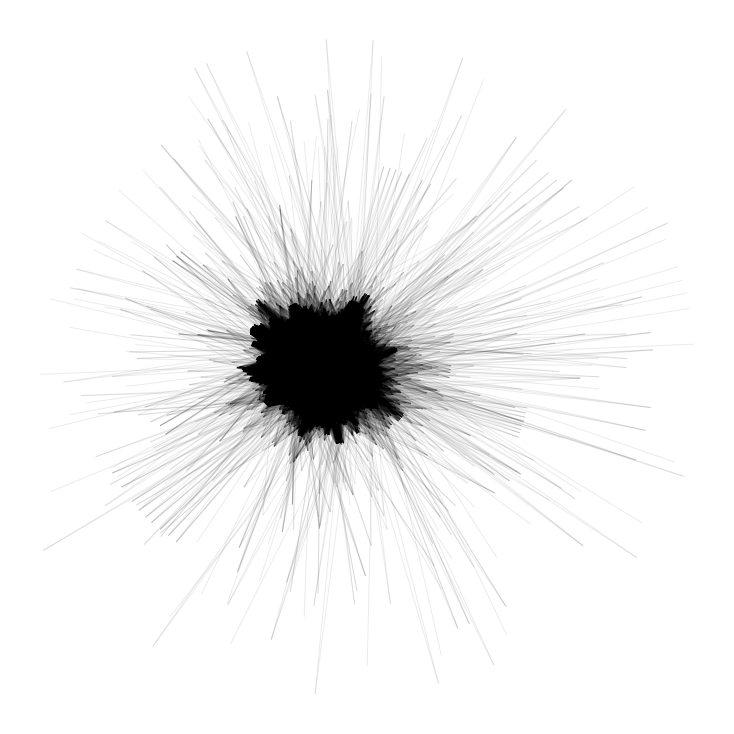
\includegraphics[width = .65\textwidth]{output_89_0.png}
    \end{figure}
    %\begin{center}
    %\adjustimage{max size={0.9\linewidth}{0.9\paperheight}}{output_89_0.png}
    %\end{center}
    { \hspace*{\fill} \\}
    
    Relembre as funções definidas anteriormente:

    \begin{tcolorbox}[breakable, size=fbox, boxrule=1pt, pad at break*=1mm,colback=cellbackground, colframe=cellborder]
\prompt{In}{incolor}{4}{\boxspacing}
\begin{Verbatim}[commandchars=\\\{\}]
\PY{k}{def} \PY{n+nf}{eigPageRank}\PY{p}{(}\PY{n}{linkMatrix}\PY{p}{)}\PY{p}{:}
    \PY{c+c1}{\PYZsh{}\PYZsh{}\PYZsh{}\PYZsh{}\PYZsh{}\PYZsh{}\PYZsh{}\PYZsh{}\PYZsh{}\PYZsh{}\PYZsh{}\PYZsh{}\PYZsh{}\PYZsh{}\PYZsh{}\PYZsh{}\PYZsh{}\PYZsh{}\PYZsh{}\PYZsh{}\PYZsh{}\PYZsh{}\PYZsh{}\PYZsh{}\PYZsh{}\PYZsh{}\PYZsh{}\PYZsh{}\PYZsh{}\PYZsh{}\PYZsh{}\PYZsh{}}
    \PY{c+c1}{\PYZsh{}\PYZsh{}\PYZsh{} PAGERANK POR AUTOVETORES \PYZsh{}\PYZsh{}\PYZsh{}}
    \PY{c+c1}{\PYZsh{}\PYZsh{}\PYZsh{}\PYZsh{}\PYZsh{}\PYZsh{}\PYZsh{}\PYZsh{}\PYZsh{}\PYZsh{}\PYZsh{}\PYZsh{}\PYZsh{}\PYZsh{}\PYZsh{}\PYZsh{}\PYZsh{}\PYZsh{}\PYZsh{}\PYZsh{}\PYZsh{}\PYZsh{}\PYZsh{}\PYZsh{}\PYZsh{}\PYZsh{}\PYZsh{}\PYZsh{}\PYZsh{}\PYZsh{}\PYZsh{}\PYZsh{}}
    
    \PY{c+c1}{\PYZsh{} Calcula os autovalores e autovetores}
    \PY{n}{eVals}\PY{p}{,} \PY{n}{eVecs} \PY{o}{=} \PY{n}{la}\PY{o}{.}\PY{n}{eig}\PY{p}{(}\PY{n}{linkMatrix}\PY{p}{)} 
    
    \PY{c+c1}{\PYZsh{} Ordena pelos autovalores}
    \PY{n}{order} \PY{o}{=} \PY{n}{np}\PY{o}{.}\PY{n}{absolute}\PY{p}{(}\PY{n}{eVals}\PY{p}{)}\PY{o}{.}\PY{n}{argsort}\PY{p}{(}\PY{p}{)}\PY{p}{[}\PY{p}{:}\PY{p}{:}\PY{o}{\PYZhy{}}\PY{l+m+mi}{1}\PY{p}{]} 
    \PY{n}{eVals} \PY{o}{=} \PY{n}{eVals}\PY{p}{[}\PY{n}{order}\PY{p}{]}
    \PY{n}{eVecs} \PY{o}{=} \PY{n}{eVecs}\PY{p}{[}\PY{p}{:}\PY{p}{,}\PY{n}{order}\PY{p}{]}
    
    \PY{c+c1}{\PYZsh{} r é o principal autovetor}
    \PY{n}{r} \PY{o}{=} \PY{n}{eVecs}\PY{p}{[}\PY{p}{:}\PY{p}{,} \PY{l+m+mi}{0}\PY{p}{]} 
    
    \PY{c+c1}{\PYZsh{} Faz o vetor somar um (e multiplica por 100 pra melhorar legibilidade).}
    \PY{k}{return} \PY{l+m+mi}{100} \PY{o}{*} \PY{n}{np}\PY{o}{.}\PY{n}{real}\PY{p}{(}\PY{n}{r} \PY{o}{/} \PY{n}{np}\PY{o}{.}\PY{n}{sum}\PY{p}{(}\PY{n}{r}\PY{p}{)}\PY{p}{)}

\PY{k}{def} \PY{n+nf}{dotPageRankD}\PY{p}{(}\PY{n}{linkMatrix}\PY{p}{,} \PY{n}{d}\PY{p}{)} \PY{p}{:}
    \PY{c+c1}{\PYZsh{}\PYZsh{}\PYZsh{}\PYZsh{}\PYZsh{}\PYZsh{}\PYZsh{}\PYZsh{}\PYZsh{}\PYZsh{}\PYZsh{}\PYZsh{}\PYZsh{}\PYZsh{}\PYZsh{}\PYZsh{}\PYZsh{}\PYZsh{}\PYZsh{}\PYZsh{}\PYZsh{}\PYZsh{}\PYZsh{}\PYZsh{}\PYZsh{}\PYZsh{}\PYZsh{}\PYZsh{}\PYZsh{}}
    \PY{c+c1}{\PYZsh{}\PYZsh{}\PYZsh{} PAGERANK POR ITERAÇÃO \PYZsh{}\PYZsh{}\PYZsh{}}
    \PY{c+c1}{\PYZsh{}\PYZsh{}\PYZsh{}\PYZsh{}\PYZsh{}\PYZsh{}\PYZsh{}\PYZsh{}\PYZsh{}\PYZsh{}\PYZsh{}\PYZsh{}\PYZsh{}\PYZsh{}\PYZsh{}\PYZsh{}\PYZsh{}\PYZsh{}\PYZsh{}\PYZsh{}\PYZsh{}\PYZsh{}\PYZsh{}\PYZsh{}\PYZsh{}\PYZsh{}\PYZsh{}\PYZsh{}\PYZsh{}}
    
    \PY{c+c1}{\PYZsh{} Armazena a quantidade de colunas}
    \PY{n}{n} \PY{o}{=} \PY{n}{linkMatrix}\PY{o}{.}\PY{n}{shape}\PY{p}{[}\PY{l+m+mi}{0}\PY{p}{]}
    
    \PY{c+c1}{\PYZsh{} Cria matriz M a partir do fator de amortecimento.}
    \PY{n}{M} \PY{o}{=} \PY{n}{d} \PY{o}{*} \PY{n}{linkMatrix} \PY{o}{+} \PY{p}{(}\PY{l+m+mi}{1}\PY{o}{\PYZhy{}}\PY{n}{d}\PY{p}{)}\PY{o}{/}\PY{n}{n} \PY{o}{*} \PY{n}{np}\PY{o}{.}\PY{n}{ones}\PY{p}{(}\PY{p}{[}\PY{n}{n}\PY{p}{,} \PY{n}{n}\PY{p}{]}\PY{p}{)}
    
    \PY{c+c1}{\PYZsh{} Vetor (n linhas 1/n × 100 cada)}
    \PY{n}{r} \PY{o}{=} \PY{l+m+mi}{100} \PY{o}{*} \PY{n}{np}\PY{o}{.}\PY{n}{ones}\PY{p}{(}\PY{n}{n}\PY{p}{)} \PY{o}{/} \PY{n}{n} 
    
    \PY{c+c1}{\PYZsh{} Altera o valor do último r}
    \PY{n}{last} \PY{o}{=} \PY{n}{r}
    
    \PY{c+c1}{\PYZsh{} Efetua o dotproduct}
    \PY{n}{r} \PY{o}{=} \PY{n}{M} \PY{o}{@} \PY{n}{r}
    
    \PY{c+c1}{\PYZsh{} Repete o processo até atender o erro arbitrário.}
    \PY{k}{while} \PY{n}{la}\PY{o}{.}\PY{n}{norm}\PY{p}{(}\PY{n}{last} \PY{o}{\PYZhy{}} \PY{n}{r}\PY{p}{)} \PY{o}{\PYZgt{}} \PY{l+m+mf}{0.01} \PY{p}{:}
        \PY{n}{last} \PY{o}{=} \PY{n}{r}
        \PY{n}{r} \PY{o}{=} \PY{n}{M} \PY{o}{@} \PY{n}{r}
    \PY{k}{return} \PY{n}{r}
\end{Verbatim}
\end{tcolorbox}

    \hypertarget{aplicando-os-algoruxedtmos}{%
\subsection{Aplicando os
algorítmos}\label{aplicando-os-algoruxedtmos}}

Vamos utilizar ambos os algorítmos apresentados em seções anteriores e
depois relacioná-los com o \emph{dataframe}.

Primeiramente, utilizando o método dos autovetores.

    \begin{tcolorbox}[breakable, size=fbox, boxrule=1pt, pad at break*=1mm,colback=cellbackground, colframe=cellborder]
\prompt{In}{incolor}{5}{\boxspacing}
\begin{Verbatim}[commandchars=\\\{\}]
\PY{o}{\PYZpc{}\PYZpc{}time}
\PY{n}{eigPR} \PY{o}{=} \PY{n}{eigPageRank}\PY{p}{(}\PY{n}{L}\PY{p}{)}
\end{Verbatim}
\end{tcolorbox}

    \begin{Verbatim}[commandchars=\\\{\}]
CPU times: user 4min 35s, sys: 1min 12s, total: 5min 47s
Wall time: 1min 8s
    \end{Verbatim}

    Em seguida, o método do \emph{dot-product}.

    \begin{tcolorbox}[breakable, size=fbox, boxrule=1pt, pad at break*=1mm,colback=cellbackground, colframe=cellborder]
\prompt{In}{incolor}{6}{\boxspacing}
\begin{Verbatim}[commandchars=\\\{\}]
\PY{o}{\PYZpc{}\PYZpc{}time}
\PY{n}{dotPR} \PY{o}{=} \PY{n}{dotPageRankD}\PY{p}{(}\PY{n}{L}\PY{p}{,} \PY{l+m+mi}{1}\PY{p}{)} \PY{c+c1}{\PYZsh{} Utilizando 1 para fazer uma comparação.}
\end{Verbatim}
\end{tcolorbox}

    \begin{Verbatim}[commandchars=\\\{\}]
CPU times: user 1.15 s, sys: 261 ms, total: 1.41 s
Wall time: 652 ms
    \end{Verbatim}

    Observe-os

    \begin{tcolorbox}[breakable, size=fbox, boxrule=1pt, pad at break*=1mm,colback=cellbackground, colframe=cellborder]
\prompt{In}{incolor}{7}{\boxspacing}
\begin{Verbatim}[commandchars=\\\{\}]
\PY{n}{eigPR}
\end{Verbatim}
\end{tcolorbox}

            \begin{tcolorbox}[breakable, size=fbox, boxrule=.5pt, pad at break*=1mm, opacityfill=0]
\prompt{Out}{outcolor}{7}{\boxspacing}
\begin{Verbatim}[commandchars=\\\{\}]
array([5.51433066e-01, 2.52080379e-02, 8.63712287e-02, {\ldots},
       1.34295455e-06, 4.37247323e-07, 4.37247323e-07])
\end{Verbatim}
\end{tcolorbox}
        
    \begin{tcolorbox}[breakable, size=fbox, boxrule=1pt, pad at break*=1mm,colback=cellbackground, colframe=cellborder]
\prompt{In}{incolor}{8}{\boxspacing}
\begin{Verbatim}[commandchars=\\\{\}]
\PY{n}{dotPR}
\end{Verbatim}
\end{tcolorbox}

            \begin{tcolorbox}[breakable, size=fbox, boxrule=.5pt, pad at break*=1mm, opacityfill=0]
\prompt{Out}{outcolor}{8}{\boxspacing}
\begin{Verbatim}[commandchars=\\\{\}]
array([3.14136484e-03, 1.43603365e-04, 4.92033500e-04, {\ldots},
       7.65044842e-09, 2.49087959e-09, 2.49087959e-09])
\end{Verbatim}
\end{tcolorbox}
        
    Os valores são, de fato, bem diferentes. Mas vamos ver quais páginas
eles apontam como mais bem ranqueadas.

Vamos, para cada um dos resultados, criar um \emph{dataframe} que une o
resultado com os sites.

    \begin{tcolorbox}[breakable, size=fbox, boxrule=1pt, pad at break*=1mm,colback=cellbackground, colframe=cellborder]
\prompt{In}{incolor}{13}{\boxspacing}
\begin{Verbatim}[commandchars=\\\{\}]
\PY{c+c1}{\PYZsh{} Removendo a coluna link do df}
\PY{n}{df2} \PY{o}{=} \PY{n}{df}\PY{o}{.}\PY{n}{drop}\PY{p}{(}\PY{n}{columns} \PY{o}{=} \PY{p}{[}\PY{l+s+s1}{\PYZsq{}}\PY{l+s+s1}{link}\PY{l+s+s1}{\PYZsq{}}\PY{p}{]}\PY{p}{)}
\PY{c+c1}{\PYZsh{} Adquirindo os sites}
\PY{n}{cols} \PY{o}{=} \PY{n+nb}{list}\PY{p}{(}\PY{n}{df2}\PY{o}{.}\PY{n}{columns}\PY{p}{)}
\end{Verbatim}
\end{tcolorbox}

    \begin{tcolorbox}[breakable, size=fbox, boxrule=1pt, pad at break*=1mm,colback=cellbackground, colframe=cellborder]
\prompt{In}{incolor}{14}{\boxspacing}
\begin{Verbatim}[commandchars=\\\{\}]
\PY{c+c1}{\PYZsh{} Método dos autovetores}
\PY{n}{rel\PYZus{}eig} \PY{o}{=} \PY{n}{pd}\PY{o}{.}\PY{n}{DataFrame}\PY{p}{(}\PY{n}{eigPR}\PY{p}{,} \PY{n}{cols}\PY{p}{)}
\end{Verbatim}
\end{tcolorbox}

    \begin{tcolorbox}[breakable, size=fbox, boxrule=1pt, pad at break*=1mm,colback=cellbackground, colframe=cellborder]
\prompt{In}{incolor}{15}{\boxspacing}
\begin{Verbatim}[commandchars=\\\{\}]
\PY{c+c1}{\PYZsh{} Método do dotproduct}
\PY{n}{rel\PYZus{}dot} \PY{o}{=} \PY{n}{pd}\PY{o}{.}\PY{n}{DataFrame}\PY{p}{(}\PY{n}{dotPR}\PY{p}{,} \PY{n}{cols}\PY{p}{)}
\end{Verbatim}
\end{tcolorbox}

    Agora podemos visualizar os primeiros 15 resultados de cada um dos
\emph{dataframes} ordenados.

    \begin{tcolorbox}[breakable, size=fbox, boxrule=1pt, pad at break*=1mm,colback=cellbackground, colframe=cellborder]
\prompt{In}{incolor}{21}{\boxspacing}
\begin{Verbatim}[commandchars=\\\{\}]
\PY{c+c1}{\PYZsh{} Método dos autovetores}
\PY{n}{rel\PYZus{}eig}\PY{o}{.}\PY{n}{sort\PYZus{}values}\PY{p}{(}\PY{l+m+mi}{0}\PY{p}{,} \PY{n}{ascending}\PY{o}{=}\PY{k+kc}{False}\PY{p}{)}\PY{p}{[}\PY{l+m+mi}{0}\PY{p}{:}\PY{l+m+mi}{15}\PY{p}{]}
\end{Verbatim}
\end{tcolorbox}

            \begin{tcolorbox}[breakable, size=fbox, boxrule=.5pt, pad at break*=1mm, opacityfill=0]
\prompt{Out}{outcolor}{21}{\boxspacing}
\begin{Verbatim}[commandchars=\\\{\}]
                                                      0
./Especial:Fontes\_de\_livros/978-0-07-709840-7  1.998577
./Emil\_Artin                                   1.800438
./Universidade\_de\_Poitiers                     1.495650
./Árvore\_(grafo)                               1.212889
./Special:BookSources/8573930217               1.044034
./Dualidade                                    0.878467
./Wikimedia                                    0.712887
./Conexidade                                   0.706123
./Função\_de\_Heaviside                          0.669221
./Função\_côncava                               0.657430
./Vetores\_de\_estado                            0.643622
./Álgebra\_linear                               0.551433
./Física\_nuclear                               0.481641
./Série\_de\_funções                             0.463906
./Tratamento\_sistemático                       0.451466
\end{Verbatim}
\end{tcolorbox}
        
    \begin{tcolorbox}[breakable, size=fbox, boxrule=1pt, pad at break*=1mm,colback=cellbackground, colframe=cellborder]
\prompt{In}{incolor}{22}{\boxspacing}
\begin{Verbatim}[commandchars=\\\{\}]
\PY{c+c1}{\PYZsh{} Método do dotproduct}
\PY{n}{rel\PYZus{}dot}\PY{o}{.}\PY{n}{sort\PYZus{}values}\PY{p}{(}\PY{l+m+mi}{0}\PY{p}{,} \PY{n}{ascending}\PY{o}{=}\PY{k+kc}{False}\PY{p}{)}\PY{p}{[}\PY{l+m+mi}{0}\PY{p}{:}\PY{l+m+mi}{15}\PY{p}{]}
\end{Verbatim}
\end{tcolorbox}

            \begin{tcolorbox}[breakable, size=fbox, boxrule=.5pt, pad at break*=1mm, opacityfill=0]
\prompt{Out}{outcolor}{22}{\boxspacing}
\begin{Verbatim}[commandchars=\\\{\}]
                                                      0
./Especial:Fontes\_de\_livros/978-0-07-709840-7  0.011385
./Emil\_Artin                                   0.010257
./Universidade\_de\_Poitiers                     0.008520
./Árvore\_(grafo)                               0.006910
./Special:BookSources/8573930217               0.005948
./Dualidade                                    0.005004
./Wikimedia                                    0.004061
./Conexidade                                   0.004023
./Função\_de\_Heaviside                          0.003812
./Função\_côncava                               0.003745
./Vetores\_de\_estado                            0.003667
./Álgebra\_linear                               0.003141
./Física\_nuclear                               0.002744
./Série\_de\_funções                             0.002643
./Tratamento\_sistemático                       0.002572
\end{Verbatim}
\end{tcolorbox}
        
    Como pode-se ver, há os mesmos resultados em ambos. Agora vamos
visualizar até que ponto eles se mantém iguais.

    \begin{tcolorbox}[breakable, size=fbox, boxrule=1pt, pad at break*=1mm,colback=cellbackground, colframe=cellborder]
\prompt{In}{incolor}{23}{\boxspacing}
\begin{Verbatim}[commandchars=\\\{\}]
\PY{c+c1}{\PYZsh{} Valores ranqueados do método dos autovalores}
\PY{n}{top\PYZus{}eig} \PY{o}{=} \PY{n}{rel\PYZus{}eig}\PY{o}{.}\PY{n}{sort\PYZus{}values}\PY{p}{(}\PY{l+m+mi}{0}\PY{p}{,} \PY{n}{ascending}\PY{o}{=}\PY{k+kc}{False}\PY{p}{)}\PY{o}{.}\PY{n}{index}
\PY{c+c1}{\PYZsh{} Valores ranqueados do método do dotproduct}
\PY{n}{top\PYZus{}dot} \PY{o}{=} \PY{n}{rel\PYZus{}dot}\PY{o}{.}\PY{n}{sort\PYZus{}values}\PY{p}{(}\PY{l+m+mi}{0}\PY{p}{,} \PY{n}{ascending}\PY{o}{=}\PY{k+kc}{False}\PY{p}{)}\PY{o}{.}\PY{n}{index}
\PY{c+c1}{\PYZsh{} Lista com as posições dos erros}
\PY{n}{errors} \PY{o}{=} \PY{p}{[}\PY{p}{]}
\PY{c+c1}{\PYZsh{} Posição inicial pra ser iterada}
\PY{n}{pos} \PY{o}{=} \PY{l+m+mi}{0}
\PY{k}{for} \PY{n}{eig}\PY{p}{,} \PY{n}{dot} \PY{o+ow}{in} \PY{n+nb}{zip}\PY{p}{(}\PY{n}{top\PYZus{}eig}\PY{p}{,} \PY{n}{top\PYZus{}dot}\PY{p}{)}\PY{p}{:}
    \PY{k}{if} \PY{n}{eig} \PY{o}{==} \PY{n}{dot}\PY{p}{:}
        \PY{n}{pos} \PY{o}{+}\PY{o}{=}\PY{l+m+mi}{1}
        \PY{k}{continue}
    \PY{k}{else}\PY{p}{:}
        \PY{n}{pos} \PY{o}{+}\PY{o}{=}\PY{l+m+mi}{1}
        \PY{n}{errors}\PY{o}{.}\PY{n}{append}\PY{p}{(}\PY{n}{pos}\PY{p}{)}
\end{Verbatim}
\end{tcolorbox}

    Agora vemos as informações sobre esses erros.

    \begin{tcolorbox}[breakable, size=fbox, boxrule=1pt, pad at break*=1mm,colback=cellbackground, colframe=cellborder]
\prompt{In}{incolor}{24}{\boxspacing}
\begin{Verbatim}[commandchars=\\\{\}]
\PY{n}{info} \PY{o}{=} \PY{l+s+sa}{f}\PY{l+s+s2}{\PYZdq{}\PYZdq{}\PYZdq{}}
\PY{l+s+s2}{Quantidade: }\PY{l+s+si}{\PYZob{}}\PY{n+nb}{len}\PY{p}{(}\PY{n}{errors}\PY{p}{)}\PY{l+s+si}{\PYZcb{}}
\PY{l+s+s2}{Menor Posição: }\PY{l+s+si}{\PYZob{}}\PY{n}{errors}\PY{p}{[}\PY{l+m+mi}{0}\PY{p}{]}\PY{l+s+si}{\PYZcb{}}
\PY{l+s+s2}{Maior Posição: }\PY{l+s+si}{\PYZob{}}\PY{n}{errors}\PY{p}{[}\PY{o}{\PYZhy{}}\PY{l+m+mi}{1}\PY{p}{]}\PY{l+s+si}{\PYZcb{}}
\PY{l+s+s2}{\PYZdq{}\PYZdq{}\PYZdq{}}
\PY{n+nb}{print}\PY{p}{(}\PY{n}{info}\PY{p}{)}
\end{Verbatim}
\end{tcolorbox}

    \begin{Verbatim}[commandchars=\\\{\}]

Quantidade: 1610
Menor Posição: 680
Maior Posição: 7059

    \end{Verbatim}

    Vendo as informações antigas, podemos ver que, para o erro menor que
0.01 arbitrário que colocamos na função, conseguimos igualdade nos
primeiros 680 resultados. De certo modo, é absurdamente raro alguém
alcançar essa página ao fazer uma busca. Portanto, é um resultado muito
satisfatório, principalmente ao comparar 679 ms com 1min 8s.

Evidentemente, é muito melhor ter uma busca extremamente rápida que
atende a imensa maioria das buscas perfeitamente que ter uma busca
extremamente demorada que mal aumenta a qualidade da busca.

Além do mais, outro fator importante que, entre a posição 680 e a
posição 7059, há somente 1610 discrepâncias. Ou seja, dentre os últimos
6379 sites, há 25\% de variação na posição. O que não é necessáriamente
ruim.

Por fim, também é possivel diminuir ainda mais o erro permitido sem
comprometer tanto a velocidade da busca.

    \hypertarget{adicionando-fator-de-aleatoriedade}{%
\subsection{Adicionando fator de
aleatoriedade}\label{adicionando-fator-de-aleatoriedade}}

Como vimos que o método do \emph{dotproduct} é eficiente, podemos
utilizá-lo com o parâmetro de aleatoriedade. O que siginifca que
assumimos que um usuário pode simplesmente escolher uma outra página do
nosso universo e acessá-la pelo campo de url. Normalmente usa-se 15\% de
probabilidade pelos motores de busca, ou seja, o fator de amortecimento
utilizado é de 85\%.

    \begin{tcolorbox}[breakable, size=fbox, boxrule=1pt, pad at break*=1mm,colback=cellbackground, colframe=cellborder]
\prompt{In}{incolor}{25}{\boxspacing}
\begin{Verbatim}[commandchars=\\\{\}]
\PY{o}{\PYZpc{}\PYZpc{}time}
\PY{n}{rdotPR} \PY{o}{=} \PY{n}{dotPageRankD}\PY{p}{(}\PY{n}{L}\PY{p}{,} \PY{l+m+mf}{.85}\PY{p}{)} \PY{c+c1}{\PYZsh{} Adicionando 15\PYZpc{} de chance dele acessar um outro site.}
\end{Verbatim}
\end{tcolorbox}

    \begin{Verbatim}[commandchars=\\\{\}]
CPU times: user 1.43 s, sys: 678 ms, total: 2.11 s
Wall time: 785 ms
    \end{Verbatim}

    Os valores aparentam ter se alterado, observe.

    \begin{tcolorbox}[breakable, size=fbox, boxrule=1pt, pad at break*=1mm,colback=cellbackground, colframe=cellborder]
\prompt{In}{incolor}{26}{\boxspacing}
\begin{Verbatim}[commandchars=\\\{\}]
\PY{n}{rdotPR}
\end{Verbatim}
\end{tcolorbox}

            \begin{tcolorbox}[breakable, size=fbox, boxrule=.5pt, pad at break*=1mm, opacityfill=0]
\prompt{Out}{outcolor}{26}{\boxspacing}
\begin{Verbatim}[commandchars=\\\{\}]
array([4.26159319e-03, 2.42903149e-04, 6.05301389e-04, {\ldots},
       2.56811254e-05, 2.57428341e-05, 2.57428341e-05])
\end{Verbatim}
\end{tcolorbox}
        
    Mas para saber a verdade, teremos que criar um \emph{dataset} a
relacionando com os links.

    \begin{tcolorbox}[breakable, size=fbox, boxrule=1pt, pad at break*=1mm,colback=cellbackground, colframe=cellborder]
\prompt{In}{incolor}{27}{\boxspacing}
\begin{Verbatim}[commandchars=\\\{\}]
\PY{n}{rel\PYZus{}rdot} \PY{o}{=} \PY{n}{pd}\PY{o}{.}\PY{n}{DataFrame}\PY{p}{(}\PY{n}{rdotPR}\PY{p}{,} \PY{n}{cols}\PY{p}{)}
\end{Verbatim}
\end{tcolorbox}

    Já podemos ver que, de fato, já há algumas alterações nas posições.

    \begin{tcolorbox}[breakable, size=fbox, boxrule=1pt, pad at break*=1mm,colback=cellbackground, colframe=cellborder]
\prompt{In}{incolor}{28}{\boxspacing}
\begin{Verbatim}[commandchars=\\\{\}]
\PY{n}{rel\PYZus{}rdot}\PY{o}{.}\PY{n}{sort\PYZus{}values}\PY{p}{(}\PY{l+m+mi}{0}\PY{p}{,} \PY{n}{ascending}\PY{o}{=}\PY{k+kc}{False}\PY{p}{)}\PY{p}{[}\PY{l+m+mi}{0}\PY{p}{:}\PY{l+m+mi}{15}\PY{p}{]}
\end{Verbatim}
\end{tcolorbox}

            \begin{tcolorbox}[breakable, size=fbox, boxrule=.5pt, pad at break*=1mm, opacityfill=0]
\prompt{Out}{outcolor}{28}{\boxspacing}
\begin{Verbatim}[commandchars=\\\{\}]
                                                      0
./Especial:Fontes\_de\_livros/978-0-07-709840-7  0.015413
./Emil\_Artin                                   0.013404
./Universidade\_de\_Poitiers                     0.011170
./Árvore\_(grafo)                               0.009325
./Special:BookSources/8573930217               0.008020
./Dualidade                                    0.006822
./Conexidade                                   0.005750
./Wikimedia                                    0.005256
./Função\_de\_Heaviside                          0.004999
./Função\_côncava                               0.004895
./Vetores\_de\_estado                            0.004504
./Álgebra\_linear                               0.004262
./Física\_nuclear                               0.003658
./Série\_de\_funções                             0.003509
./Tratamento\_sistemático                       0.003494
\end{Verbatim}
\end{tcolorbox}
        
    Agora, usaremos da mesma lógica aplicada entre os dois métodos para
verificar as discrepâncias.

    \begin{tcolorbox}[breakable, size=fbox, boxrule=1pt, pad at break*=1mm,colback=cellbackground, colframe=cellborder]
\prompt{In}{incolor}{29}{\boxspacing}
\begin{Verbatim}[commandchars=\\\{\}]
\PY{c+c1}{\PYZsh{} Valores ranqueados do método do dotproduct sem aleatoriedade}
\PY{n}{top\PYZus{}dot} \PY{o}{=} \PY{n}{rel\PYZus{}dot}\PY{o}{.}\PY{n}{sort\PYZus{}values}\PY{p}{(}\PY{l+m+mi}{0}\PY{p}{,} \PY{n}{ascending}\PY{o}{=}\PY{k+kc}{False}\PY{p}{)}\PY{o}{.}\PY{n}{index}
\PY{c+c1}{\PYZsh{} Valores ranqueados do método do dotproduct com aleatoriedade}
\PY{n}{top\PYZus{}rdot} \PY{o}{=} \PY{n}{rel\PYZus{}rdot}\PY{o}{.}\PY{n}{sort\PYZus{}values}\PY{p}{(}\PY{l+m+mi}{0}\PY{p}{,} \PY{n}{ascending}\PY{o}{=}\PY{k+kc}{False}\PY{p}{)}\PY{o}{.}\PY{n}{index}
\PY{c+c1}{\PYZsh{} Lista com as posições das diferenças}
\PY{n}{diff} \PY{o}{=} \PY{p}{[}\PY{p}{]}
\PY{c+c1}{\PYZsh{} Posição inicial pra ser iterada}
\PY{n}{idx} \PY{o}{=} \PY{l+m+mi}{0}
\PY{k}{for} \PY{n}{eig}\PY{p}{,} \PY{n}{dot} \PY{o+ow}{in} \PY{n+nb}{zip}\PY{p}{(}\PY{n}{top\PYZus{}dot}\PY{p}{,} \PY{n}{top\PYZus{}rdot}\PY{p}{)}\PY{p}{:}
    \PY{k}{if} \PY{n}{eig} \PY{o}{==} \PY{n}{dot}\PY{p}{:}
        \PY{n}{idx} \PY{o}{+}\PY{o}{=}\PY{l+m+mi}{1}
        \PY{k}{continue}
    \PY{k}{else}\PY{p}{:}
        \PY{n}{idx} \PY{o}{+}\PY{o}{=}\PY{l+m+mi}{1}
        \PY{n}{diff}\PY{o}{.}\PY{n}{append}\PY{p}{(}\PY{n}{idx}\PY{p}{)}
\end{Verbatim}
\end{tcolorbox}

    \begin{tcolorbox}[breakable, size=fbox, boxrule=1pt, pad at break*=1mm,colback=cellbackground, colframe=cellborder]
\prompt{In}{incolor}{30}{\boxspacing}
\begin{Verbatim}[commandchars=\\\{\}]
\PY{n}{info} \PY{o}{=} \PY{l+s+sa}{f}\PY{l+s+s2}{\PYZdq{}\PYZdq{}\PYZdq{}}
\PY{l+s+s2}{Quantidade: }\PY{l+s+si}{\PYZob{}}\PY{n+nb}{len}\PY{p}{(}\PY{n}{diff}\PY{p}{)}\PY{l+s+si}{\PYZcb{}}
\PY{l+s+s2}{Menor Posição: }\PY{l+s+si}{\PYZob{}}\PY{n}{diff}\PY{p}{[}\PY{l+m+mi}{0}\PY{p}{]}\PY{l+s+si}{\PYZcb{}}
\PY{l+s+s2}{Maior Posição: }\PY{l+s+si}{\PYZob{}}\PY{n}{diff}\PY{p}{[}\PY{o}{\PYZhy{}}\PY{l+m+mi}{1}\PY{p}{]}\PY{l+s+si}{\PYZcb{}}
\PY{l+s+s2}{\PYZdq{}\PYZdq{}\PYZdq{}}
\PY{n+nb}{print}\PY{p}{(}\PY{n}{info}\PY{p}{)}
\end{Verbatim}
\end{tcolorbox}

    \begin{Verbatim}[commandchars=\\\{\}]

Quantidade: 7019
Menor Posição: 7
Maior Posição: 7060

    \end{Verbatim}

    Como se pode ver, embora as primeiras posições não sejam alteradas, há
uma variação enorme entre os dois. É importante esclarecer que nesse
caso não se tratam de erros, pois o método utilizado adota essa
aleatoriedade como verdade. Mas vejamos se os 60 primeiros são
parecidos, por exemplo:

    \begin{tcolorbox}[breakable, size=fbox, boxrule=1pt, pad at break*=1mm,colback=cellbackground, colframe=cellborder]
\prompt{In}{incolor}{37}{\boxspacing}
\begin{Verbatim}[commandchars=\\\{\}]
\PY{n}{top\PYZus{}60\PYZus{}dot} \PY{o}{=} \PY{n}{rel\PYZus{}dot}\PY{o}{.}\PY{n}{sort\PYZus{}values}\PY{p}{(}\PY{l+m+mi}{0}\PY{p}{,} \PY{n}{ascending}\PY{o}{=}\PY{k+kc}{False}\PY{p}{)}\PY{o}{.}\PY{n}{index}\PY{p}{[}\PY{p}{:}\PY{l+m+mi}{60}\PY{p}{]}
\PY{n}{top\PYZus{}60\PYZus{}rdot} \PY{o}{=} \PY{n}{rel\PYZus{}rdot}\PY{o}{.}\PY{n}{sort\PYZus{}values}\PY{p}{(}\PY{l+m+mi}{0}\PY{p}{,} \PY{n}{ascending}\PY{o}{=}\PY{k+kc}{False}\PY{p}{)}\PY{o}{.}\PY{n}{index}\PY{p}{[}\PY{p}{:}\PY{l+m+mi}{60}\PY{p}{]}

\PY{c+c1}{\PYZsh{} Diferença simétrica.}
\PY{n+nb}{len}\PY{p}{(}\PY{n}{top\PYZus{}60\PYZus{}dot}\PY{p}{[}\PY{o}{\PYZti{}}\PY{n}{top\PYZus{}60\PYZus{}rdot}\PY{o}{.}\PY{n}{isin}\PY{p}{(}\PY{n}{top\PYZus{}60\PYZus{}dot}\PY{p}{)}\PY{p}{]}\PY{p}{)}
\end{Verbatim}
\end{tcolorbox}

            \begin{tcolorbox}[breakable, size=fbox, boxrule=.5pt, pad at break*=1mm, opacityfill=0]
\prompt{Out}{outcolor}{37}{\boxspacing}
\begin{Verbatim}[commandchars=\\\{\}]
7
\end{Verbatim}
\end{tcolorbox}
        
    Somente 7 de variação, ou seja, embora aparente uma grande mudança,
dentre os 60 primeiros sites, a maioria das mudanças são entre esse
próprio conjunto.

    \hypertarget{conclusuxe3o}{%
\section{Conclusão}\label{conclusuxe3o}}

Por fim, temos que esse algoritmo é, de fato, muito importante para a
computação. Além de ser eficiente tanto em velocidade quanto em ranquear
de forma satisfatória, ele ser alimentado por conceitos conhecidos de
Álgebra Linear é algo extremamente benéfico de se estudar. Conseguimos,
de modo geral, aplicar diversos conceitos aprendidos não somente ao
longo da disciplina, mas unir ferramentas abordadas ao longo do curso.

Fomos muito felizes em conseguir aplicar o projeto em um conjunto de
dados totalmente único e original. Inclusive, é de nosso interesse
manter público esse método de aquisição de dados. Trabalhamos em
conjunto utilizando o JupyterLab hospedado pela EMAp e versionamento
Git/GitHub. A maior dificuldade foi lidar com as quase 50 milhões de
entradas em nossa matriz, que nos forçava esperar por algum tempo para
receber resultados de alguns testes. Entretanto, essa quantidade
relativamente grande de dados nos permitiu enxergar de fato o quão
rápido o \emph{Power Method} é em relação ao \emph{Eigen Method}. Enfim,
esperamos que o trabalho tenha sido satisfatório. Sinta-se a vontade para
acessar \href{https://github.com/adamesalles/LinearAlgebra-PageRank}{nosso repositório no GitHub.}
Principalmente pelo pdf limitar a visualização de objetos abordados por nós no trabalho como,
por exemplo, o \emph{dataframe} utilizado.

\hypertarget{referuxeancias}{%
\section*{Referências}\label{referuxeancias}}

Patel, Kamlesh. (2014). Improve Page Rank Algorithm using Normalized
Technique. International Journal of Data Warehousing and Mining. 4.
42-47.

David Austin Grand Valley State University. (2006). How Google Finds
Your Needle in the Web's Haystack. The American Mathematical Society.
Disponível em:
\url{http://www.ams.org/publicoutreach/feature-column/fcarc-pagerank}.

Wikipédia, a enciclopédia livre. (2021). PageRank. Disponível em:
\url{https://en.wikipedia.org/wiki/PageRank}.


    % Add a bibliography block to the postdoc
    
    
    
\end{document}
